\documentclass[compress]{beamer}
\usepackage{ifthen,verbatim}

\title{Systematics Studies \\ which become Debugging Sessions}
\author{Jim Pivarski}
\institute{Texas A\&M University}
\date{30 July, 2007}

\newcommand{\isnote}{}
\xdefinecolor{lightyellow}{rgb}{1.,1.,0.25}
\xdefinecolor{darkblue}{rgb}{0.1,0.1,0.7}

%% %% Uncomment this to get annotations
%% \def\notes{\addtocounter{page}{-1}
%%            \renewcommand{\isnote}{*}
%% 	   \beamertemplateshadingbackground{lightyellow}{white}
%%            \begin{frame}
%%            \frametitle{Notes for the previous page (page \insertpagenumber)}
%%            \itemize}
%% \def\endnotes{\enditemize
%% 	      \end{frame}
%%               \beamertemplateshadingbackground{white}{white}
%%               \renewcommand{\isnote}{}}

%% Uncomment this to not get annotations
\def\notes{\comment}
\def\endnotes{\endcomment}

\setbeamertemplate{navigation symbols}{}
\setbeamertemplate{headline}{\includegraphics[height=1 cm]{../cmslogo} \hspace{0.1 cm} \includegraphics[height=1 cm]{../tamulogo} \hfill
\begin{minipage}{5.5 cm}
\vspace{-0.75 cm} \small
\begin{center}
\ifthenelse{\equal{\insertpagenumber}{1}}{}{\textcolor{blue}{\insertsection}}
\end{center}
\end{minipage} \hfill
\begin{minipage}{4.5 cm}
\vspace{-0.75 cm} \small
\begin{flushright}
\ifthenelse{\equal{\insertpagenumber}{1}}{}{Jim Pivarski \hspace{0.5 cm} \insertpagenumber\isnote/\pageref{numpages}}
\end{flushright}
\end{minipage}\mbox{\hspace{0.2 cm}}}

\begin{document}
\frame{\titlepage}

\begin{notes}
\item This is the annotated version of my talk.
\item If you want the version that I am presenting, download the one
labeled ``slides'' on Indico (or just ignore these yellow pages).
\item The annotated version is provided for extra detail and a written
record of comments that I intend to make orally.
\item Yellow notes refer to the content on the {\it previous} page.
\item All other slides are identical for the two versions.
\end{notes}

\begin{frame}
\frametitle{What I've been up to}
\begin{itemize}\setlength{\itemsep}{0.1 cm}
\item Using sample of 5000 $Z\to\mu\mu$ events in 1\_5\_2
\begin{center}
\tiny /castor/cern.ch/user/p/pivarski/AlCaRecoMu/1\_5\_2/zmumu.root
\end{center}

\item (Not using 15$\times$ larger sample of single muons\ldots yet)
\begin{center}
\tiny /castor/cern.ch/user/p/pivarski/AlCaRecoMu/1\_5\_2/singlemu/*
\end{center}

\item Fully realistic misalignments:
\begin{itemize}\setlength{\itemsep}{0.05 cm}
  \item CSC Layers $\Delta x = 191$ $\mu$m, $\Delta y = 335$ $\mu$m, $\Delta \phi_z = 40$ $\mu$rad
  \item All Chambers $\Delta x = \Delta y = \Delta z = 3$ mm, \\ \mbox{ } \hfill $\Delta \phi_x = \Delta \phi_y = \Delta \phi_z = 1$ mrad
  \item Disks/wheels $\Delta x = \Delta y = \Delta z = 1$ cm, \\ \mbox{ } \hfill $\Delta \phi_x = \Delta \phi_y = \Delta \phi_z = 1$ mrad
  \item Tracker 10 pb$^{-1}$ scenario
\end{itemize}

\item Align muon system to tracker with globalMuons: $x$, $y$, $\phi_z$

\item Aligning disks and wheels with 2000 $Z \to \mu\mu$ (0.36 pb$^{-1}$)

\item \underline{WORK IN PROGRESS!!!}

\end{itemize}
\end{frame}

\begin{frame}
\frametitle{Nominal case (everything as specified on slide 2)}
\begin{center}
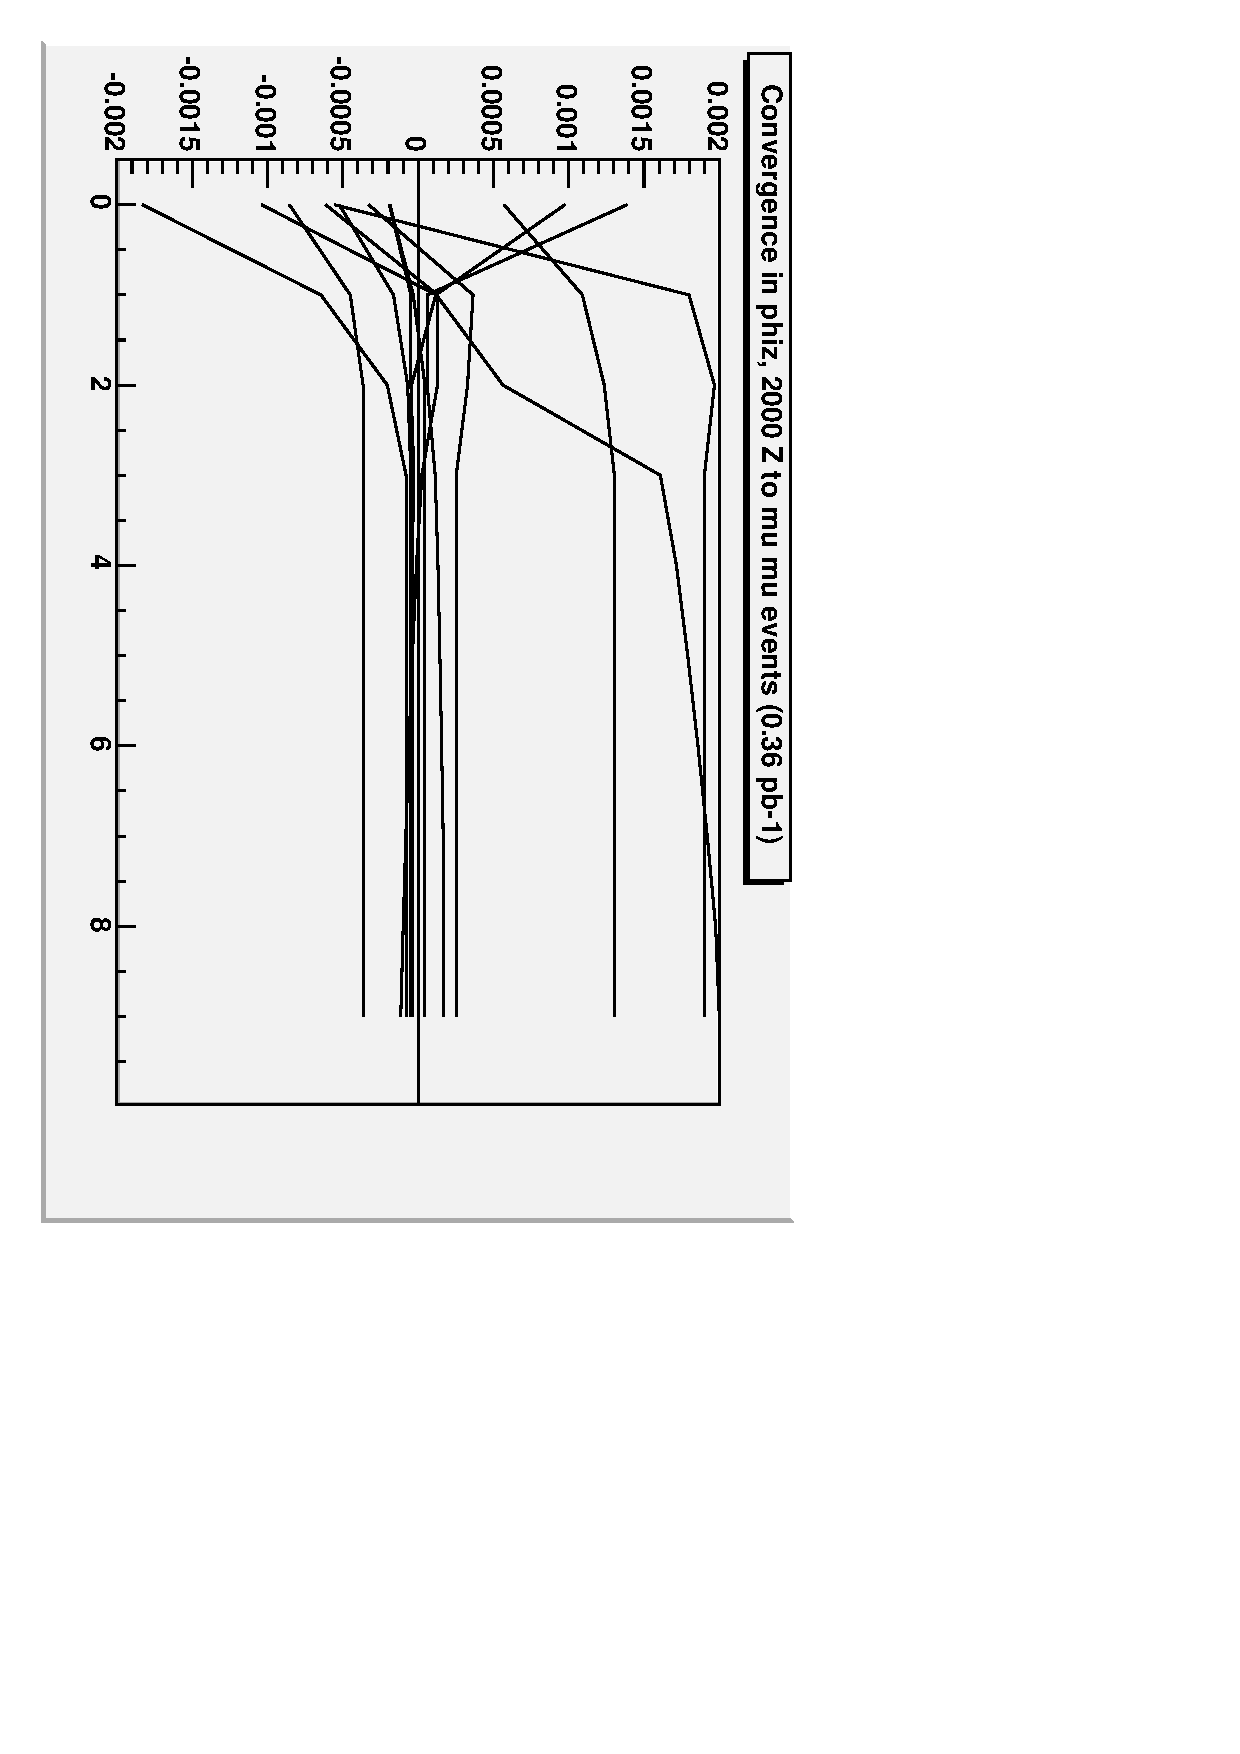
\includegraphics[height=0.8\linewidth, angle=90]{phiz_conv_2000.pdf}
\end{center}
\end{frame}

\begin{frame}
\frametitle{Effect of fitting weights on residuals}
\begin{center}
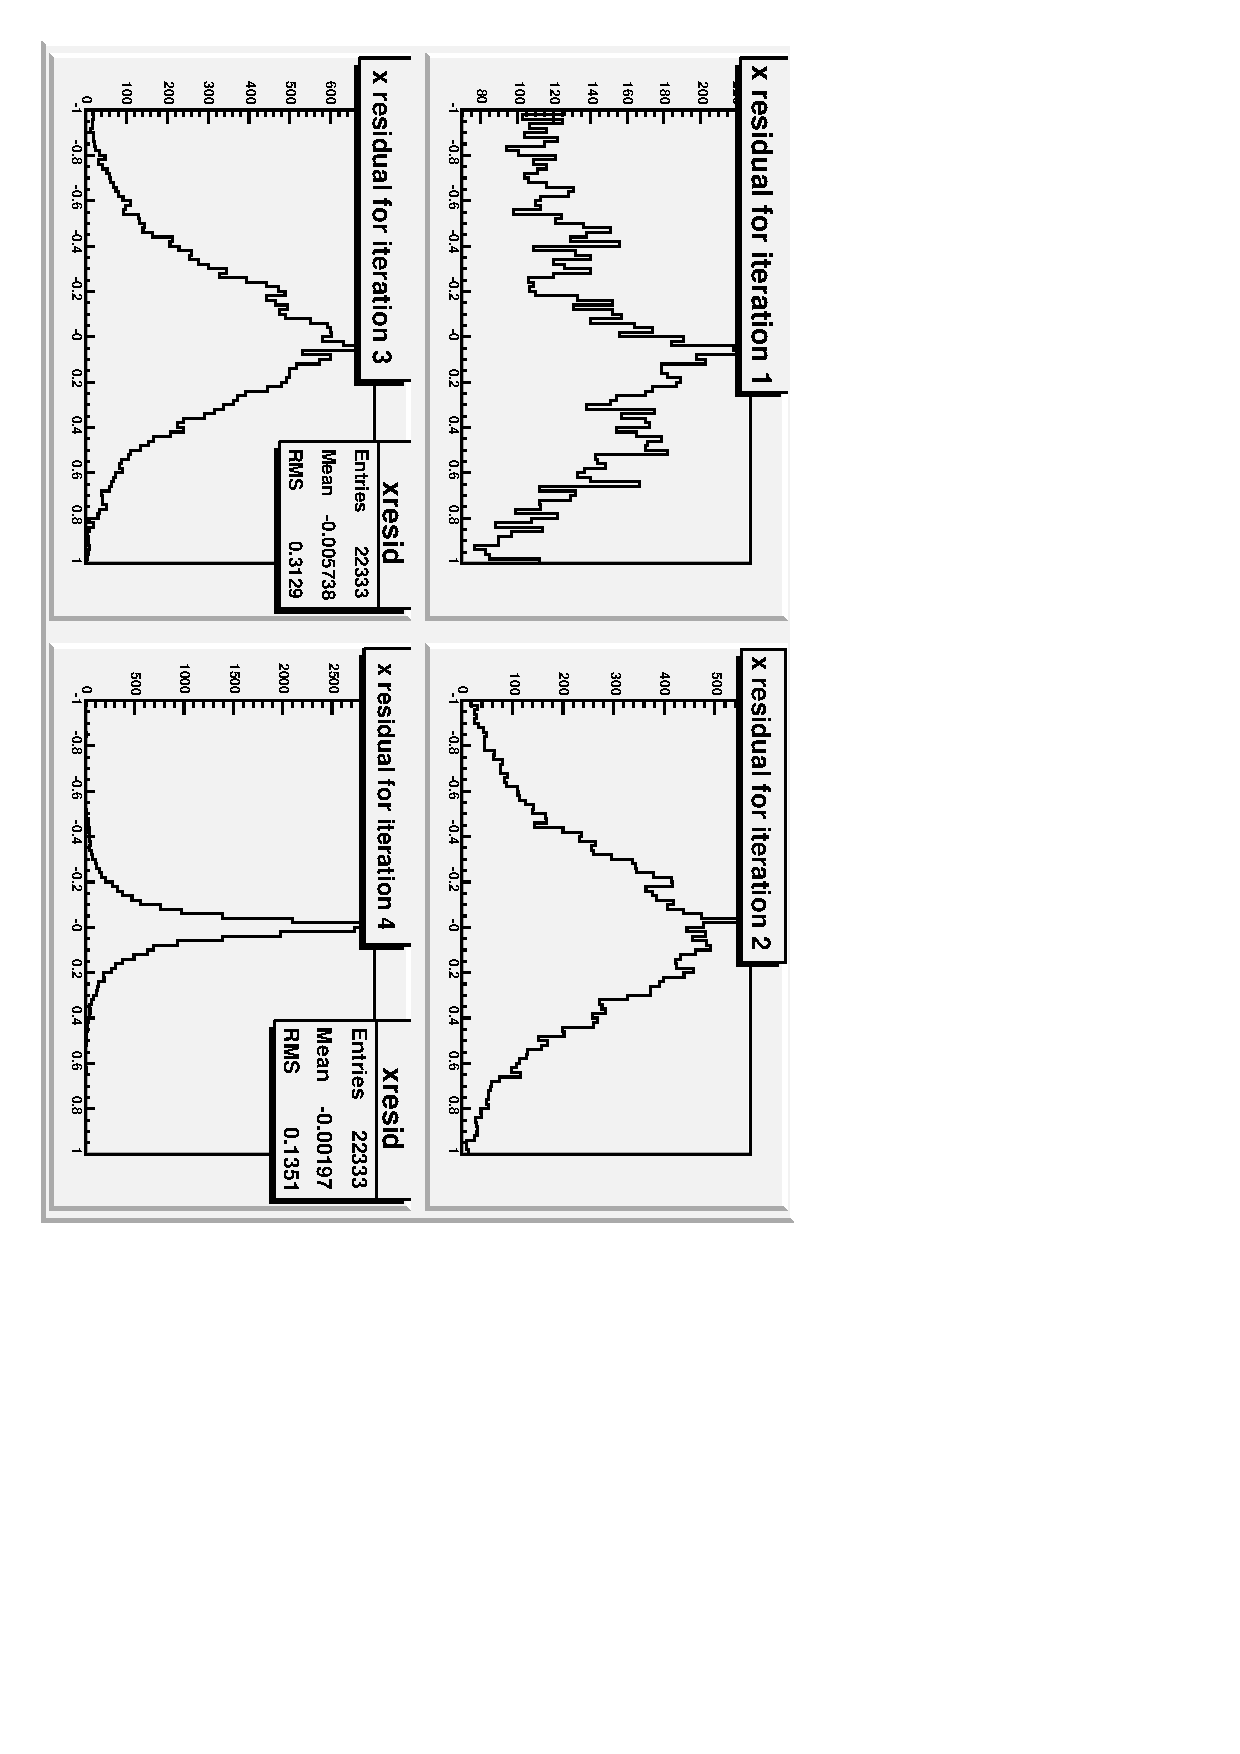
\includegraphics[height=0.7\linewidth, angle=90]{residuals_by_iteration.pdf}
\end{center}

\vfill

Alignment parameter errors (APEs) in muon system fall exponentially,
drop below hit uncertainty between steps 3 and 4.

\vspace{0.2 cm}

Error used in fit = $\sqrt{(\mbox{APE})^2 + (\mbox{hit uncertainty})^2}$

\end{frame}

\begin{frame}
\frametitle{Nominal case again (just a reminder)}
\begin{center}
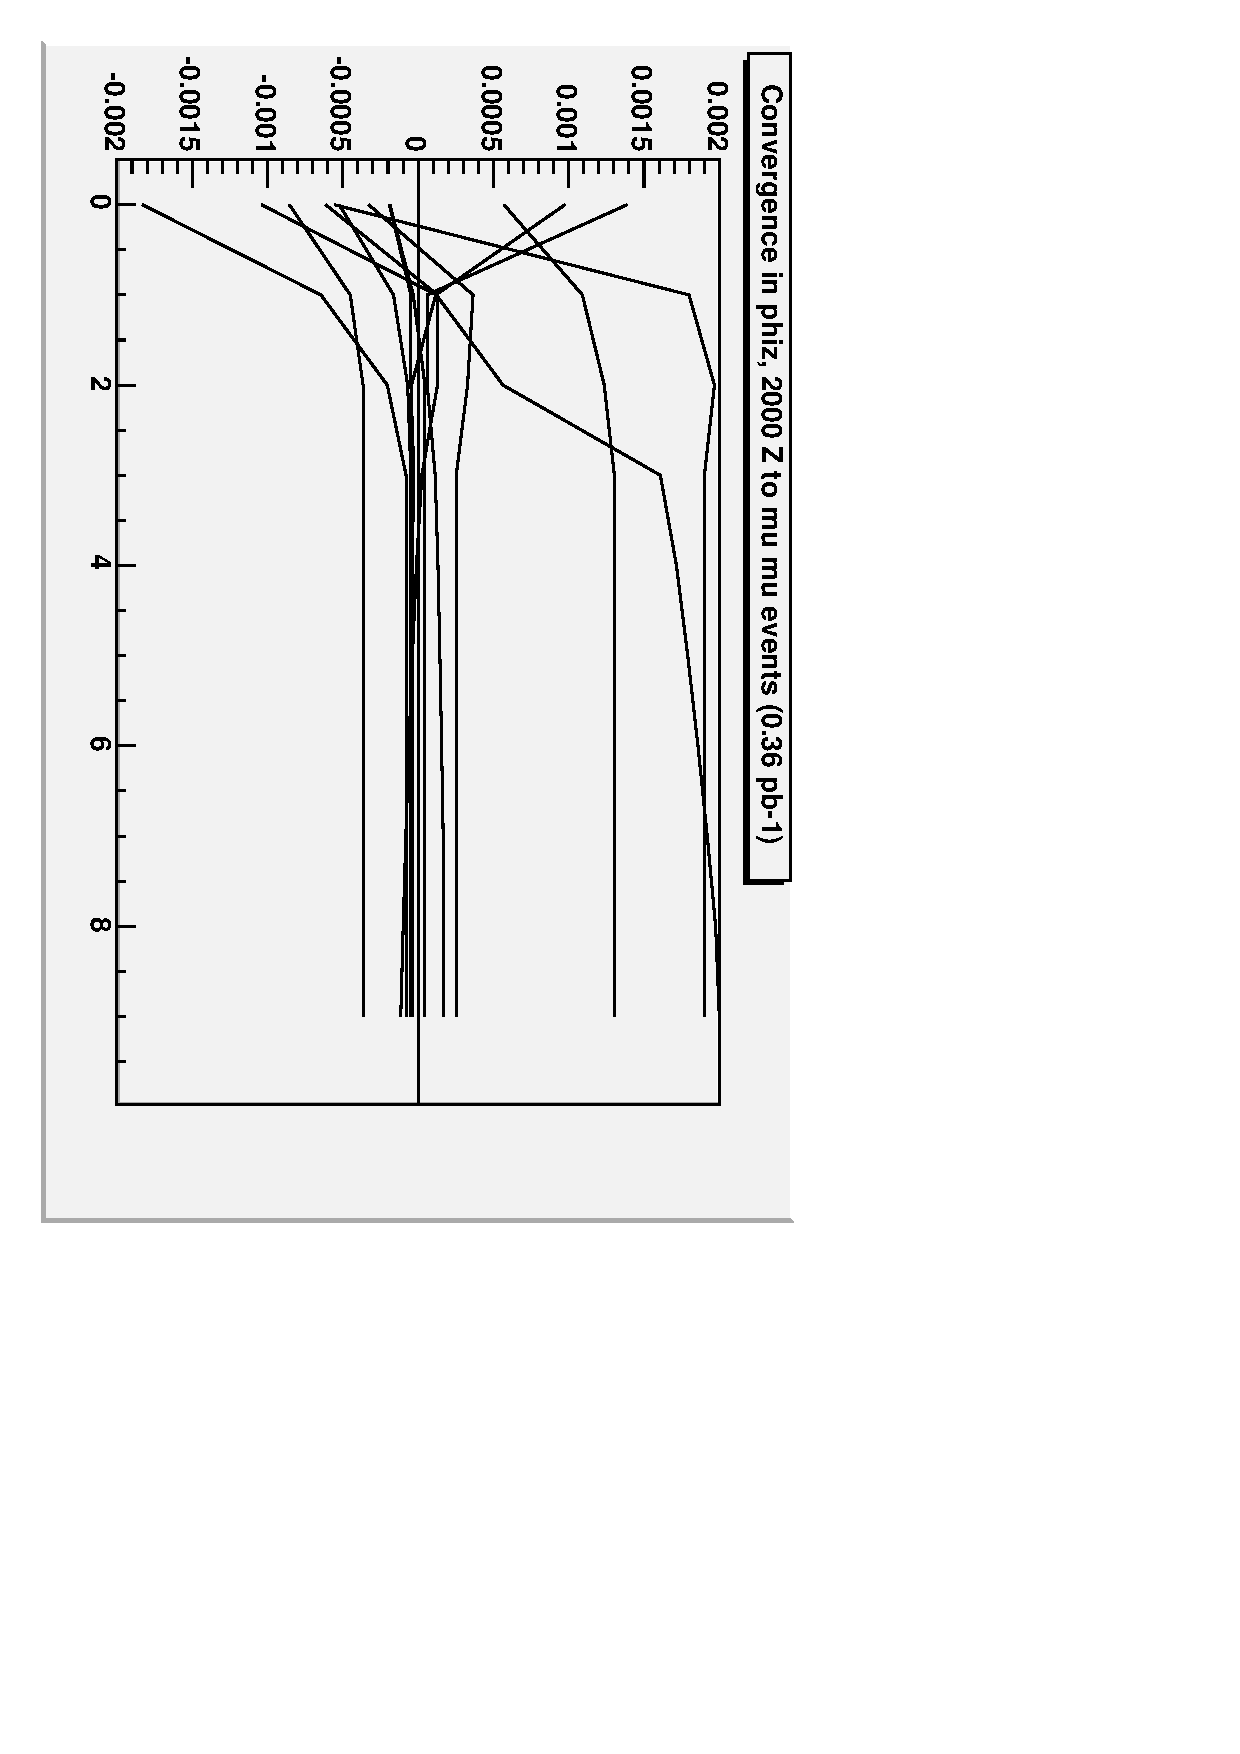
\includegraphics[height=0.8\linewidth, angle=90]{phiz_conv_2000.pdf}
\end{center}
\end{frame}

\begin{frame}
\frametitle{Ideal tracker}
\begin{center}
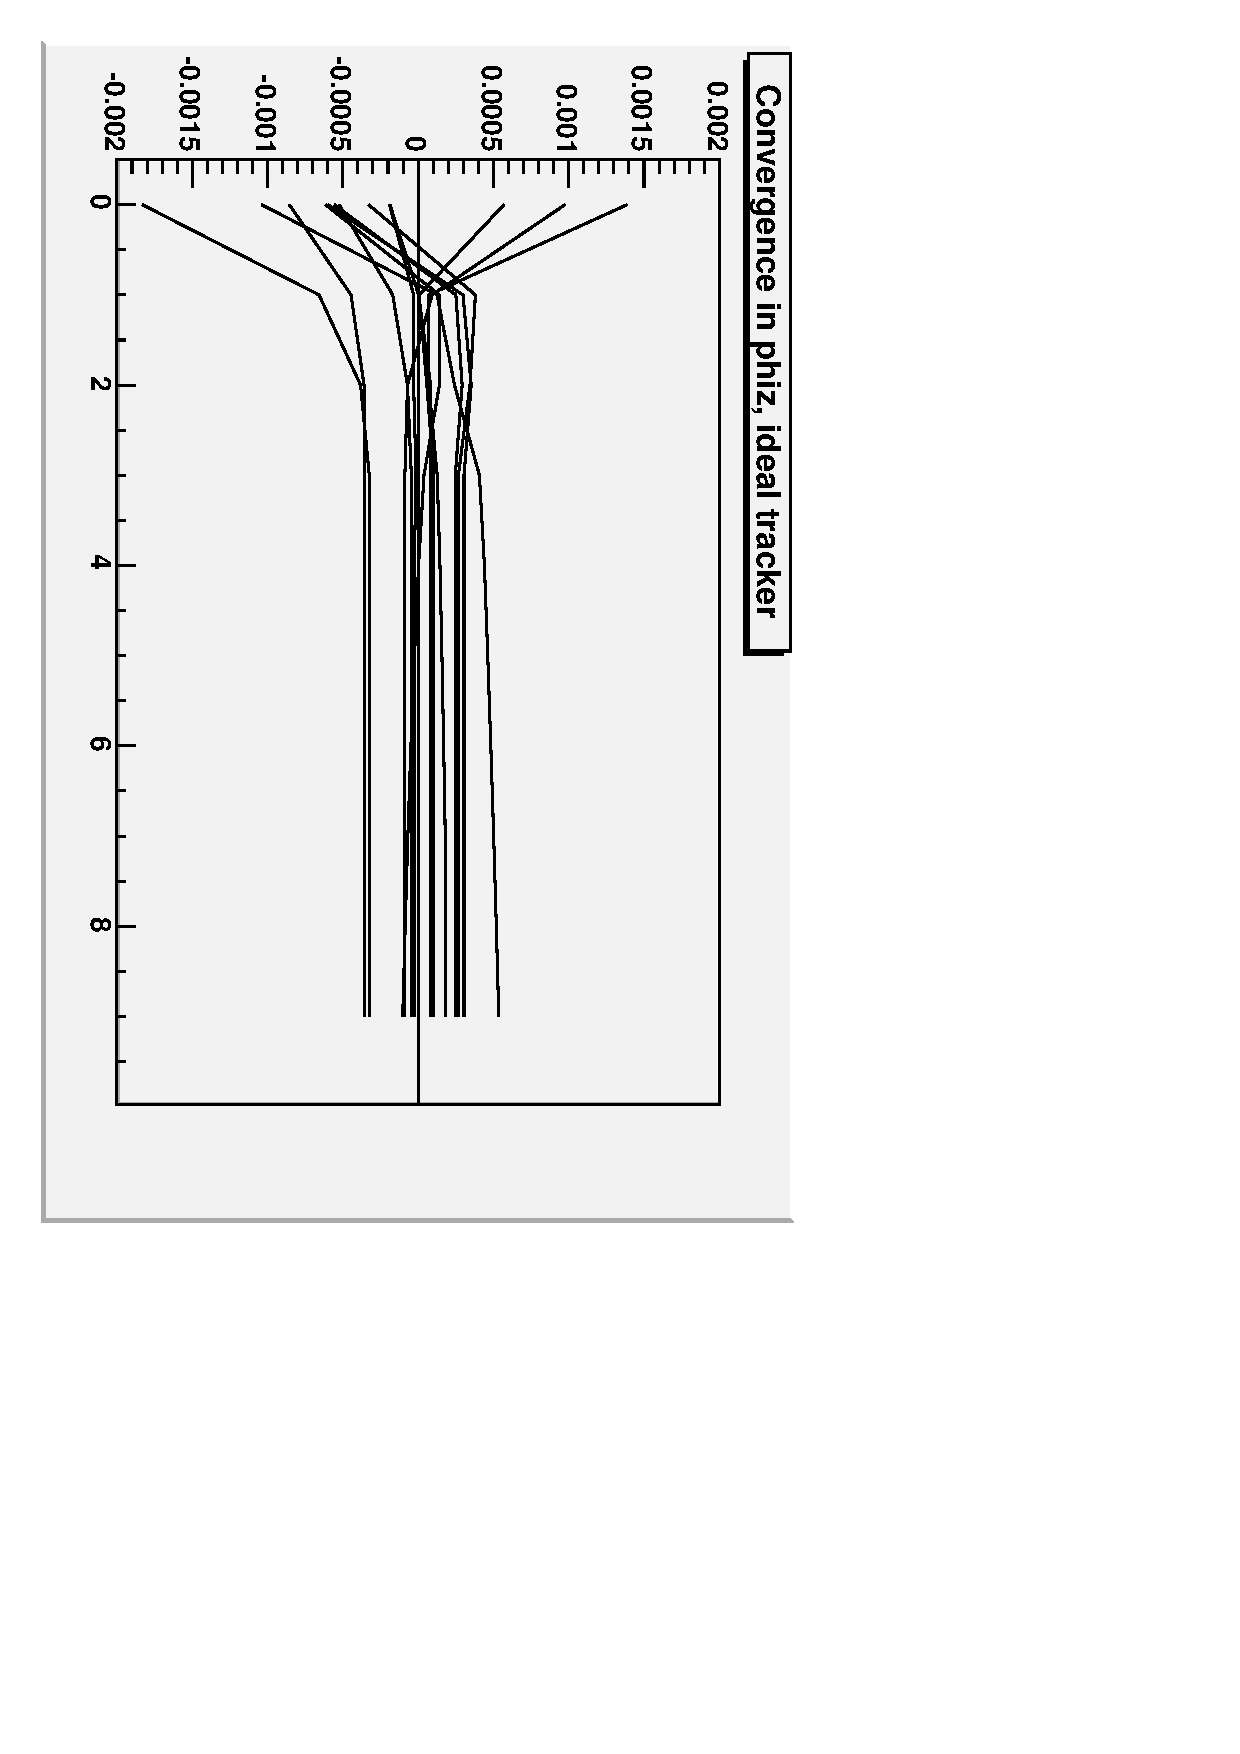
\includegraphics[height=0.8\linewidth, angle=90]{phiz_conv_ideal_tracker.pdf}
\end{center}
\end{frame}

\begin{frame}
\frametitle{Roll the tracker (ideal $+$ 1 mrad rotation)}
\begin{center}
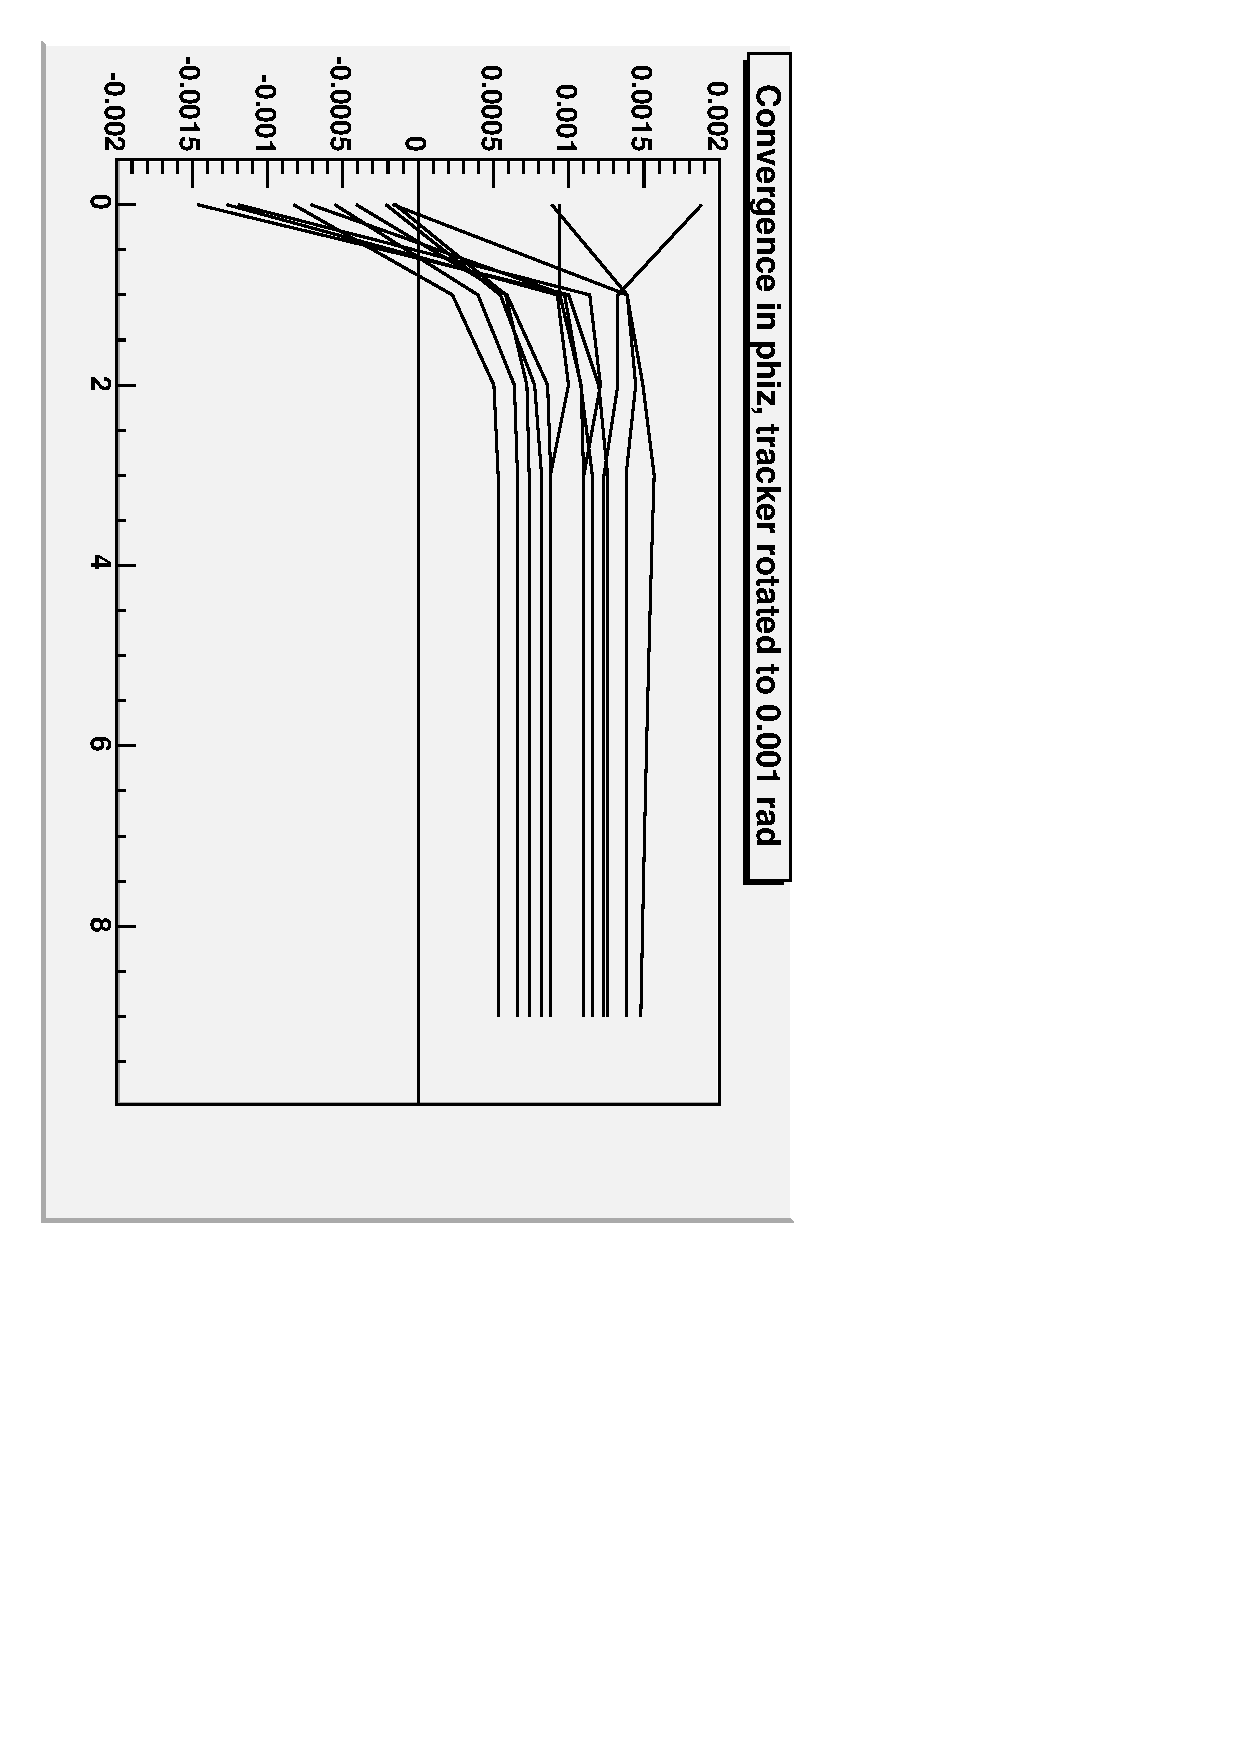
\includegraphics[height=0.8\linewidth, angle=90]{phiz_conv_barrel_roll.pdf}
\end{center}

Lessons: (1) pixel barrel (PXB) center is not on the beamline \\

\textcolor{white}{Lessons:} (2) {\it make sure to exclude RPC hits from track fitter!!!} \\

\end{frame}

\begin{frame}
\frametitle{Ideal tracker again (just a reminder)}
\begin{center}
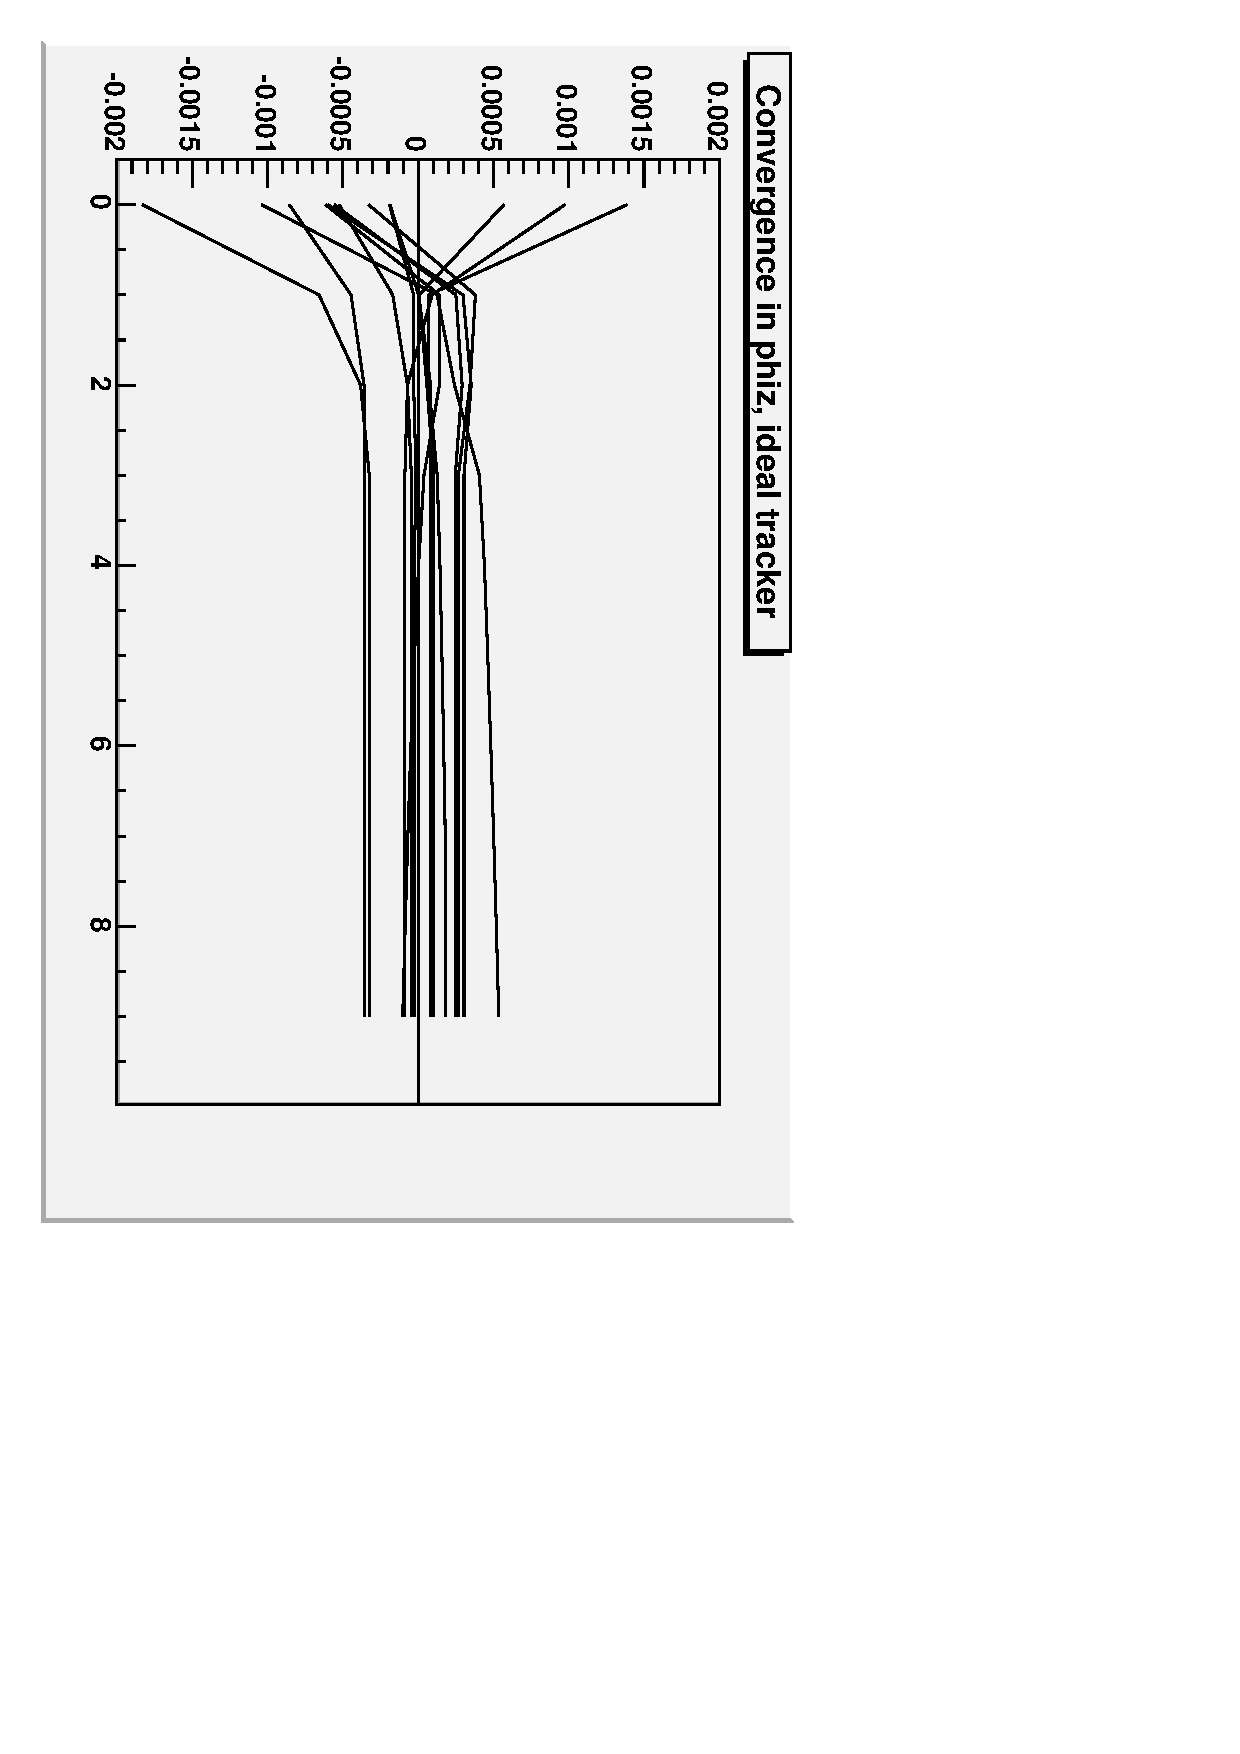
\includegraphics[height=0.8\linewidth, angle=90]{phiz_conv_ideal_tracker.pdf}
\end{center}
\end{frame}

\begin{frame}
\frametitle{Nominal 10 pb$^{-1}$ tracker scenario again (just a reminder)}
\begin{center}
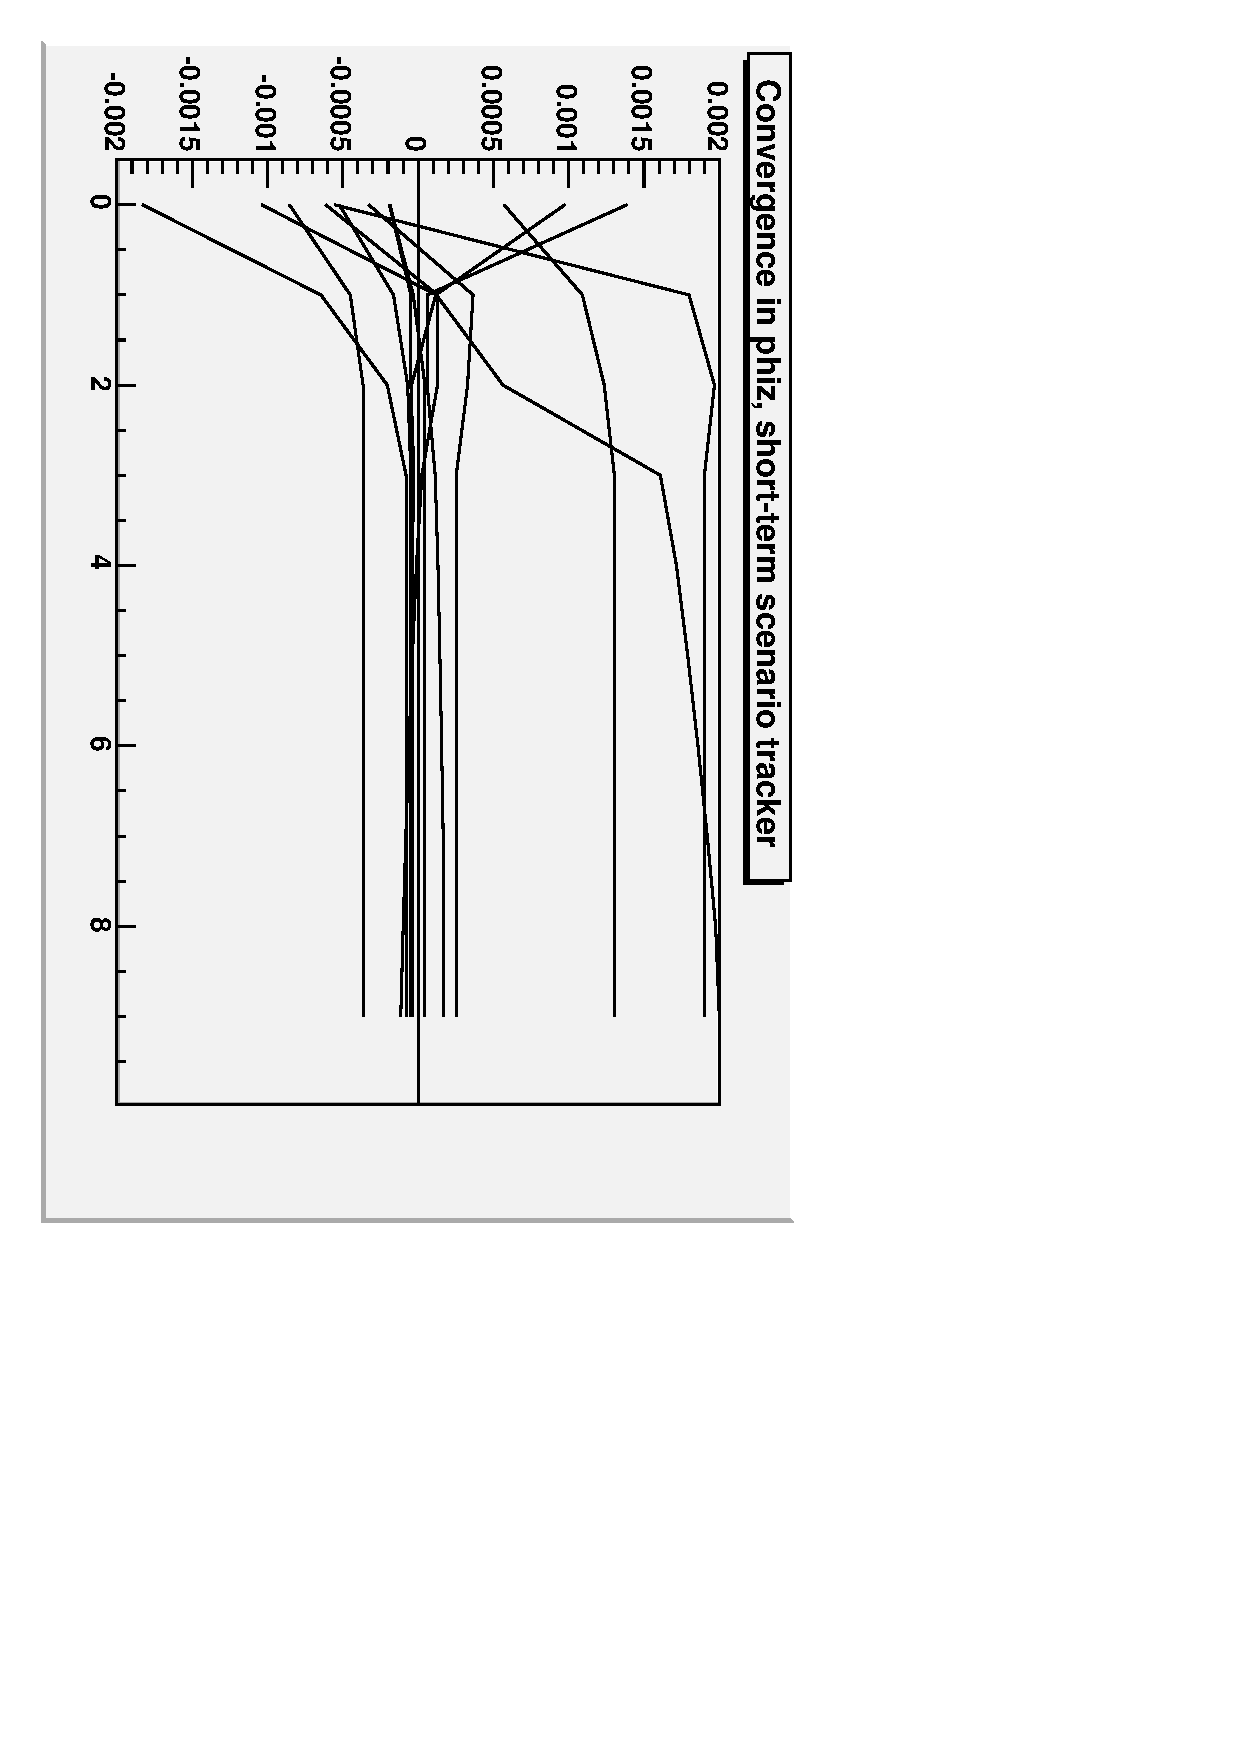
\includegraphics[height=0.8\linewidth, angle=90]{phiz_conv_nominal.pdf}
\end{center}
\end{frame}

\begin{frame}
\frametitle{Twice the tracker misalignment (?)}
\begin{center}
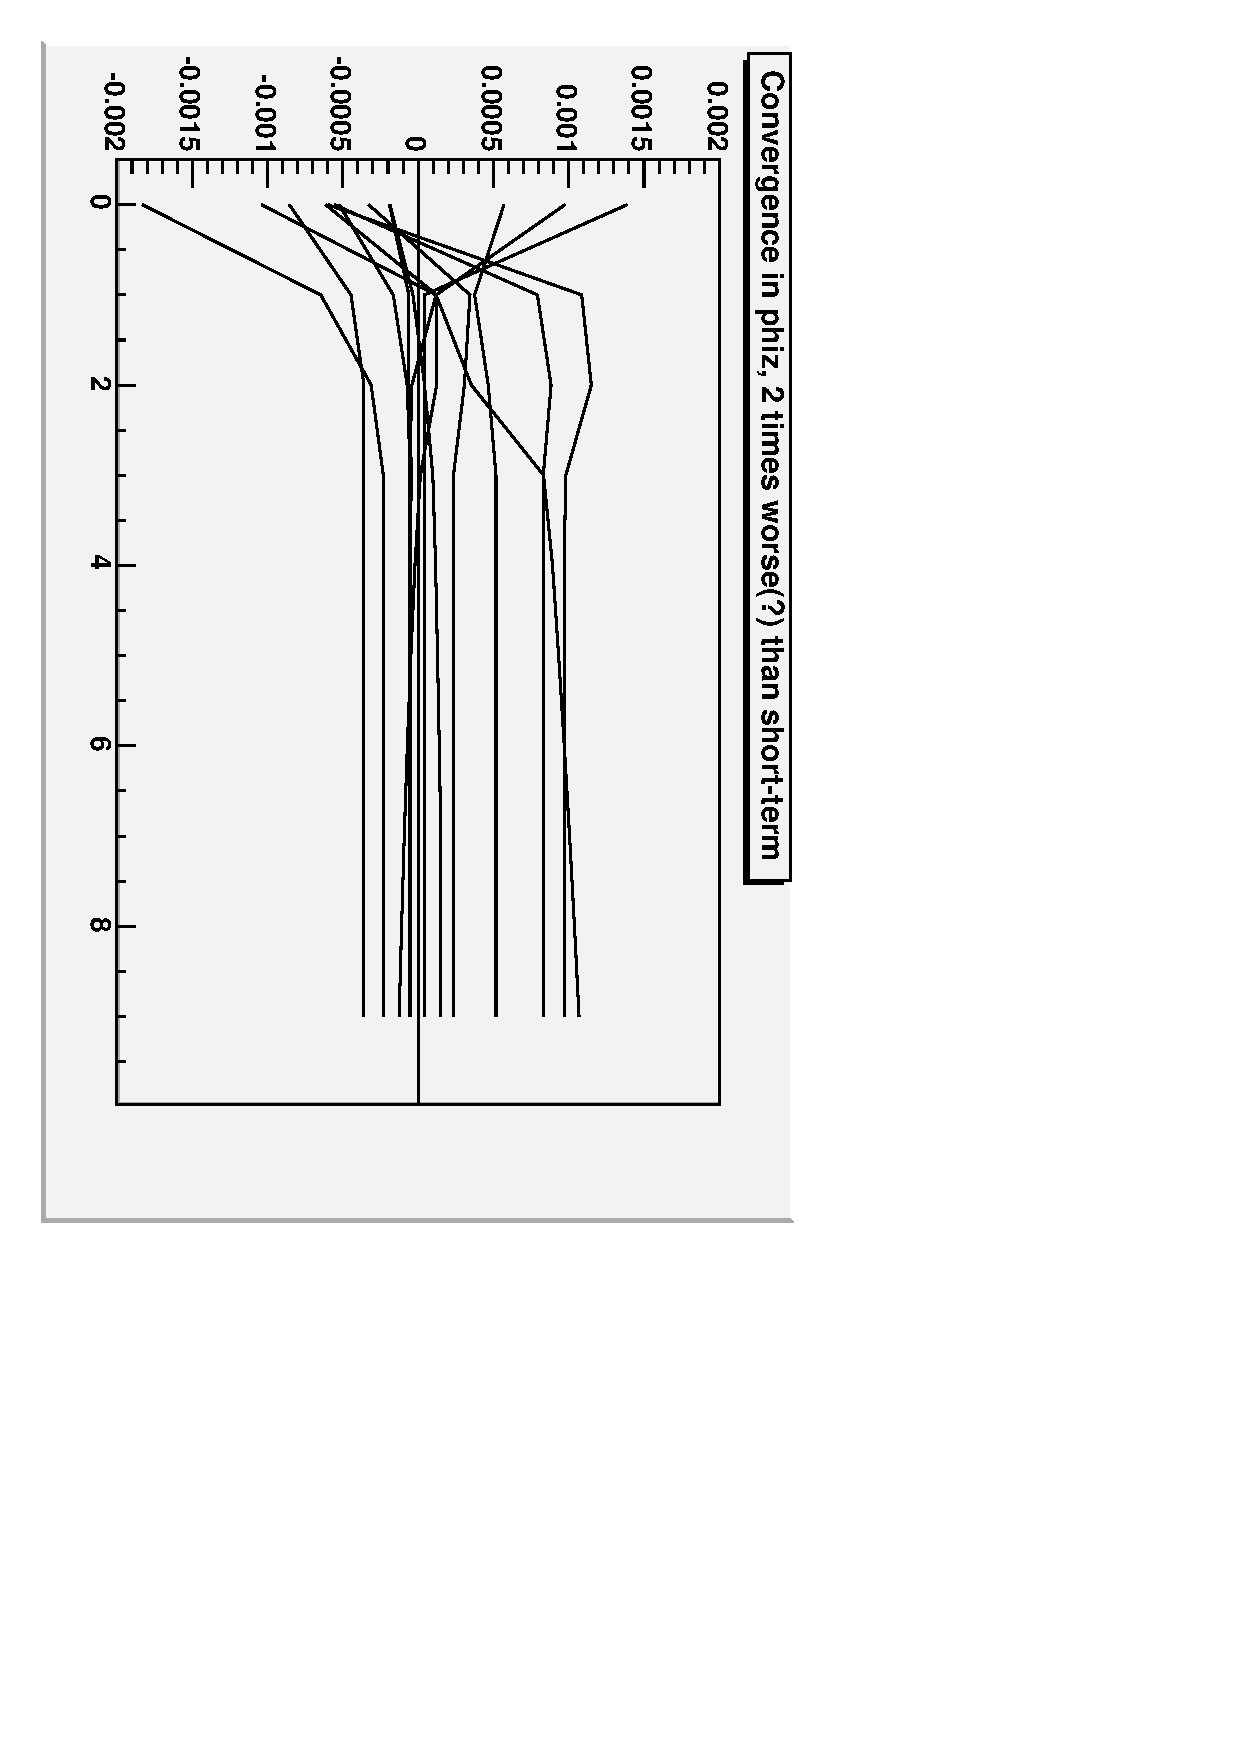
\includegraphics[height=0.8\linewidth, angle=90]{phiz_conv_times2.pdf}
\end{center}
\end{frame}

\begin{frame}
\frametitle{Five times the tracker misalignment (??)}
\begin{center}
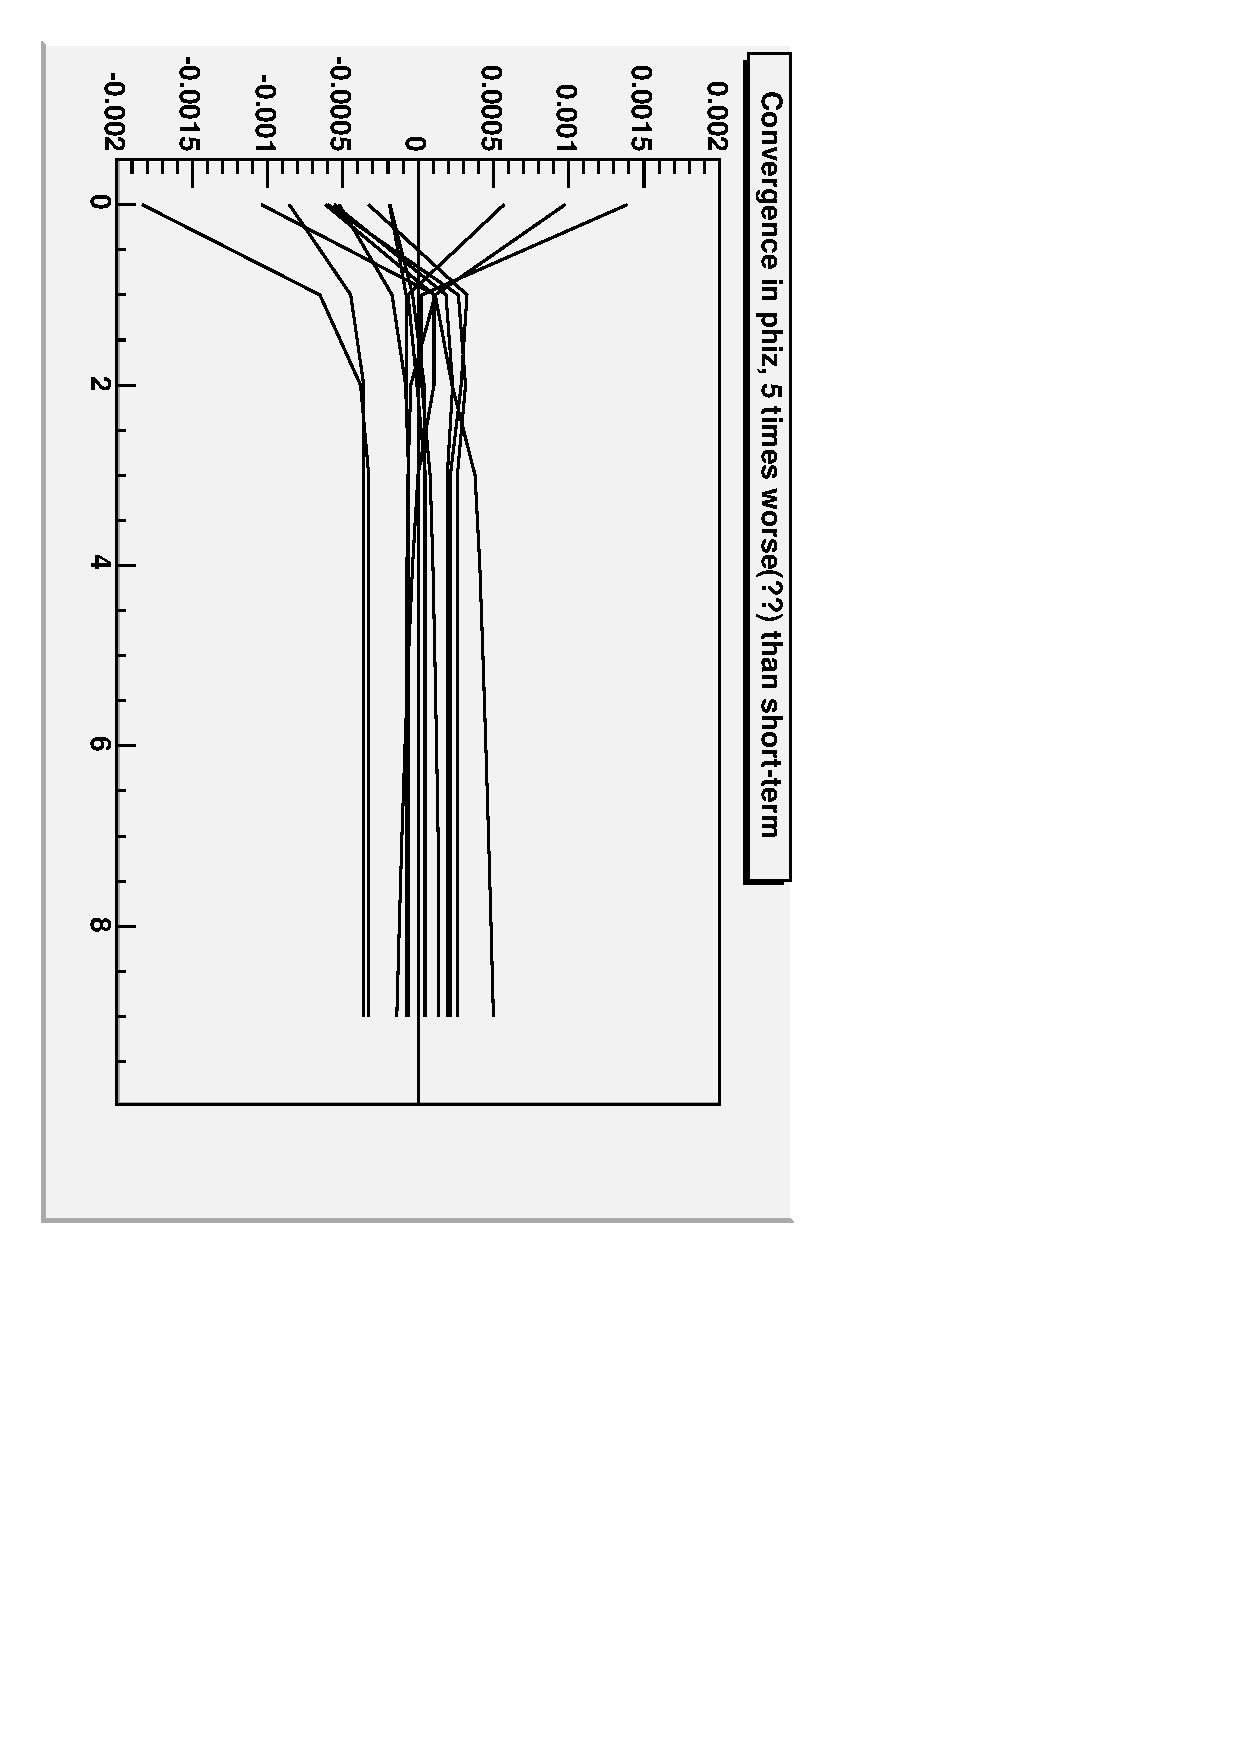
\includegraphics[height=0.8\linewidth, angle=90]{phiz_conv_times5.pdf}
\end{center}
\end{frame}

\begin{frame}
\frametitle{Ten times the tracker misalignment (?!??!??!???)}
\begin{center}
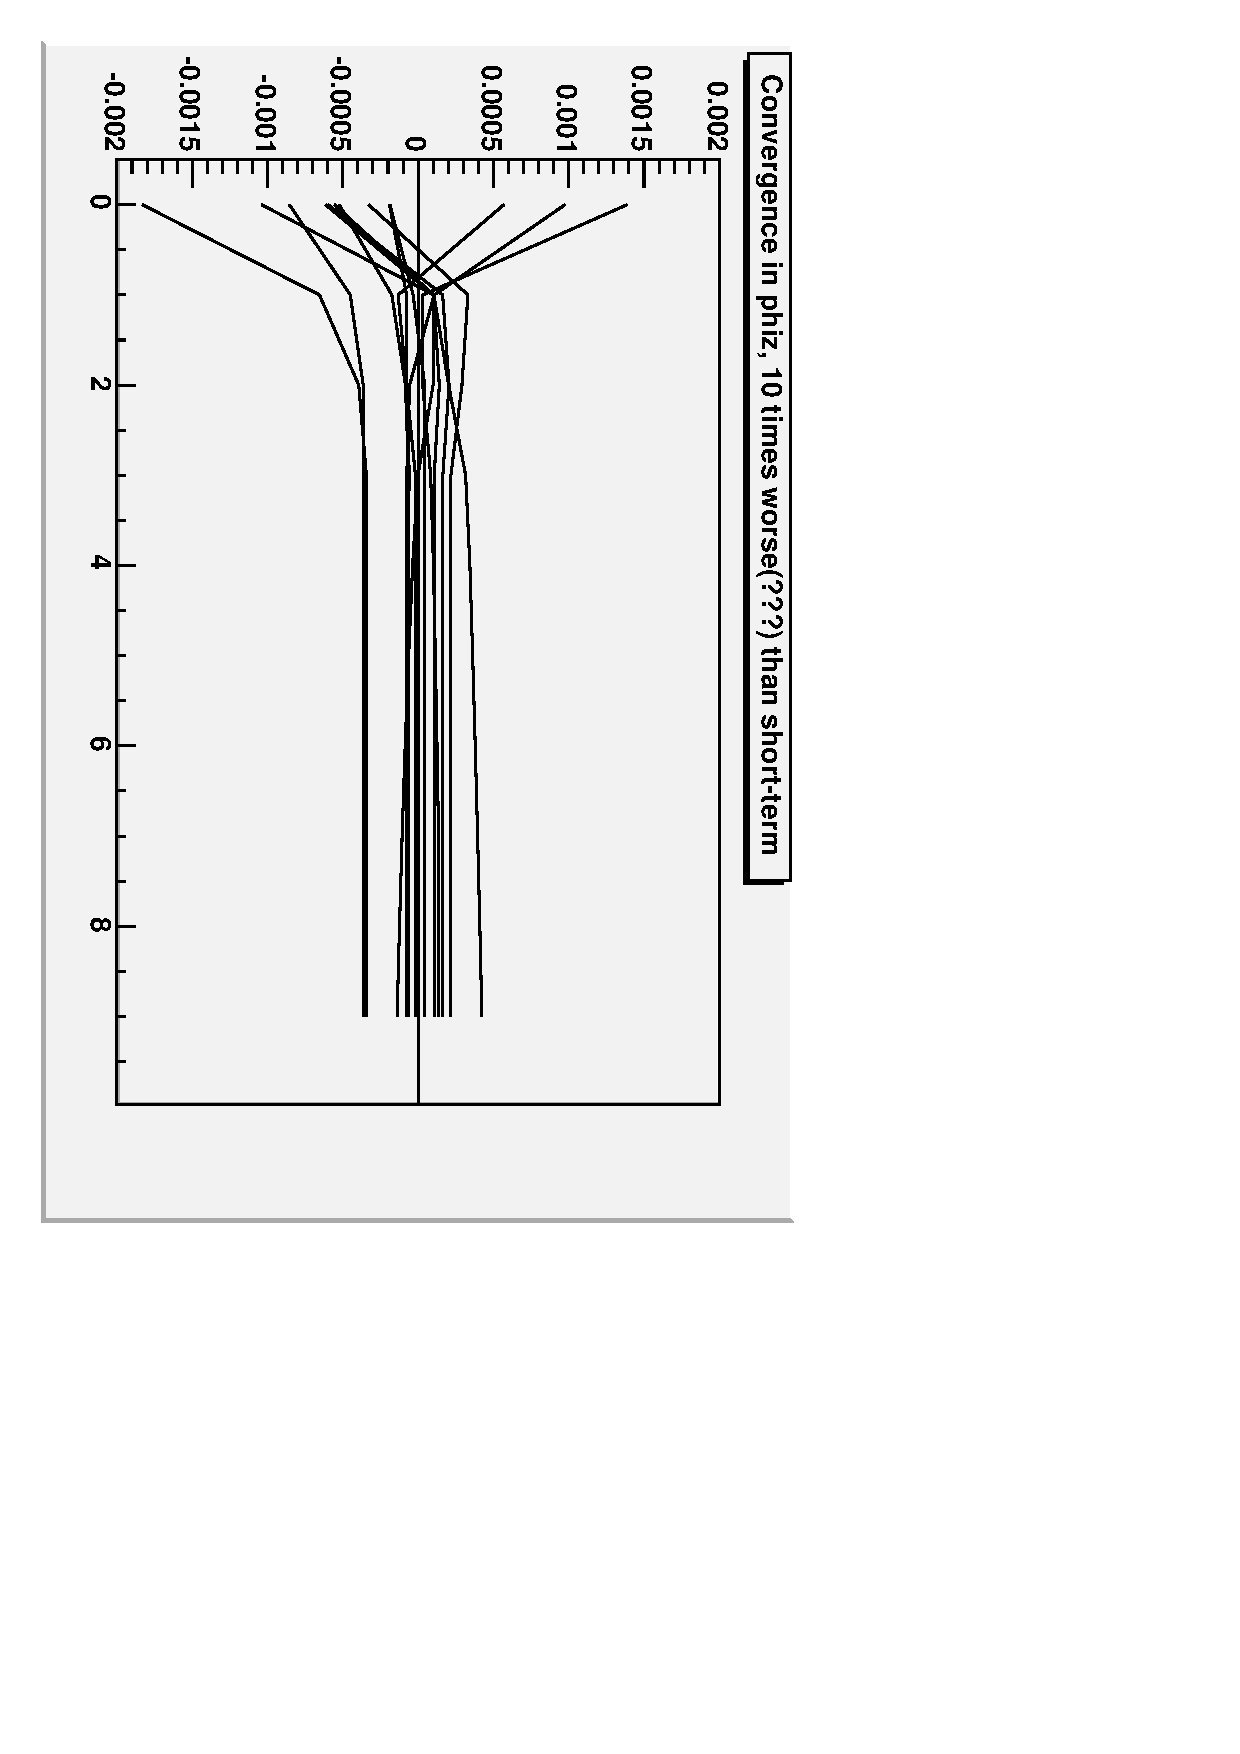
\includegraphics[height=0.8\linewidth, angle=90]{phiz_conv_times10.pdf}
\end{center}
\end{frame}

\begin{frame}
\frametitle{No, I don't understand this yet.}

RMS of 13 disk/wheels times 10 trials, randomizing muon alignment with
each trial (but not tracker alignment).

\vfill
\begin{center}
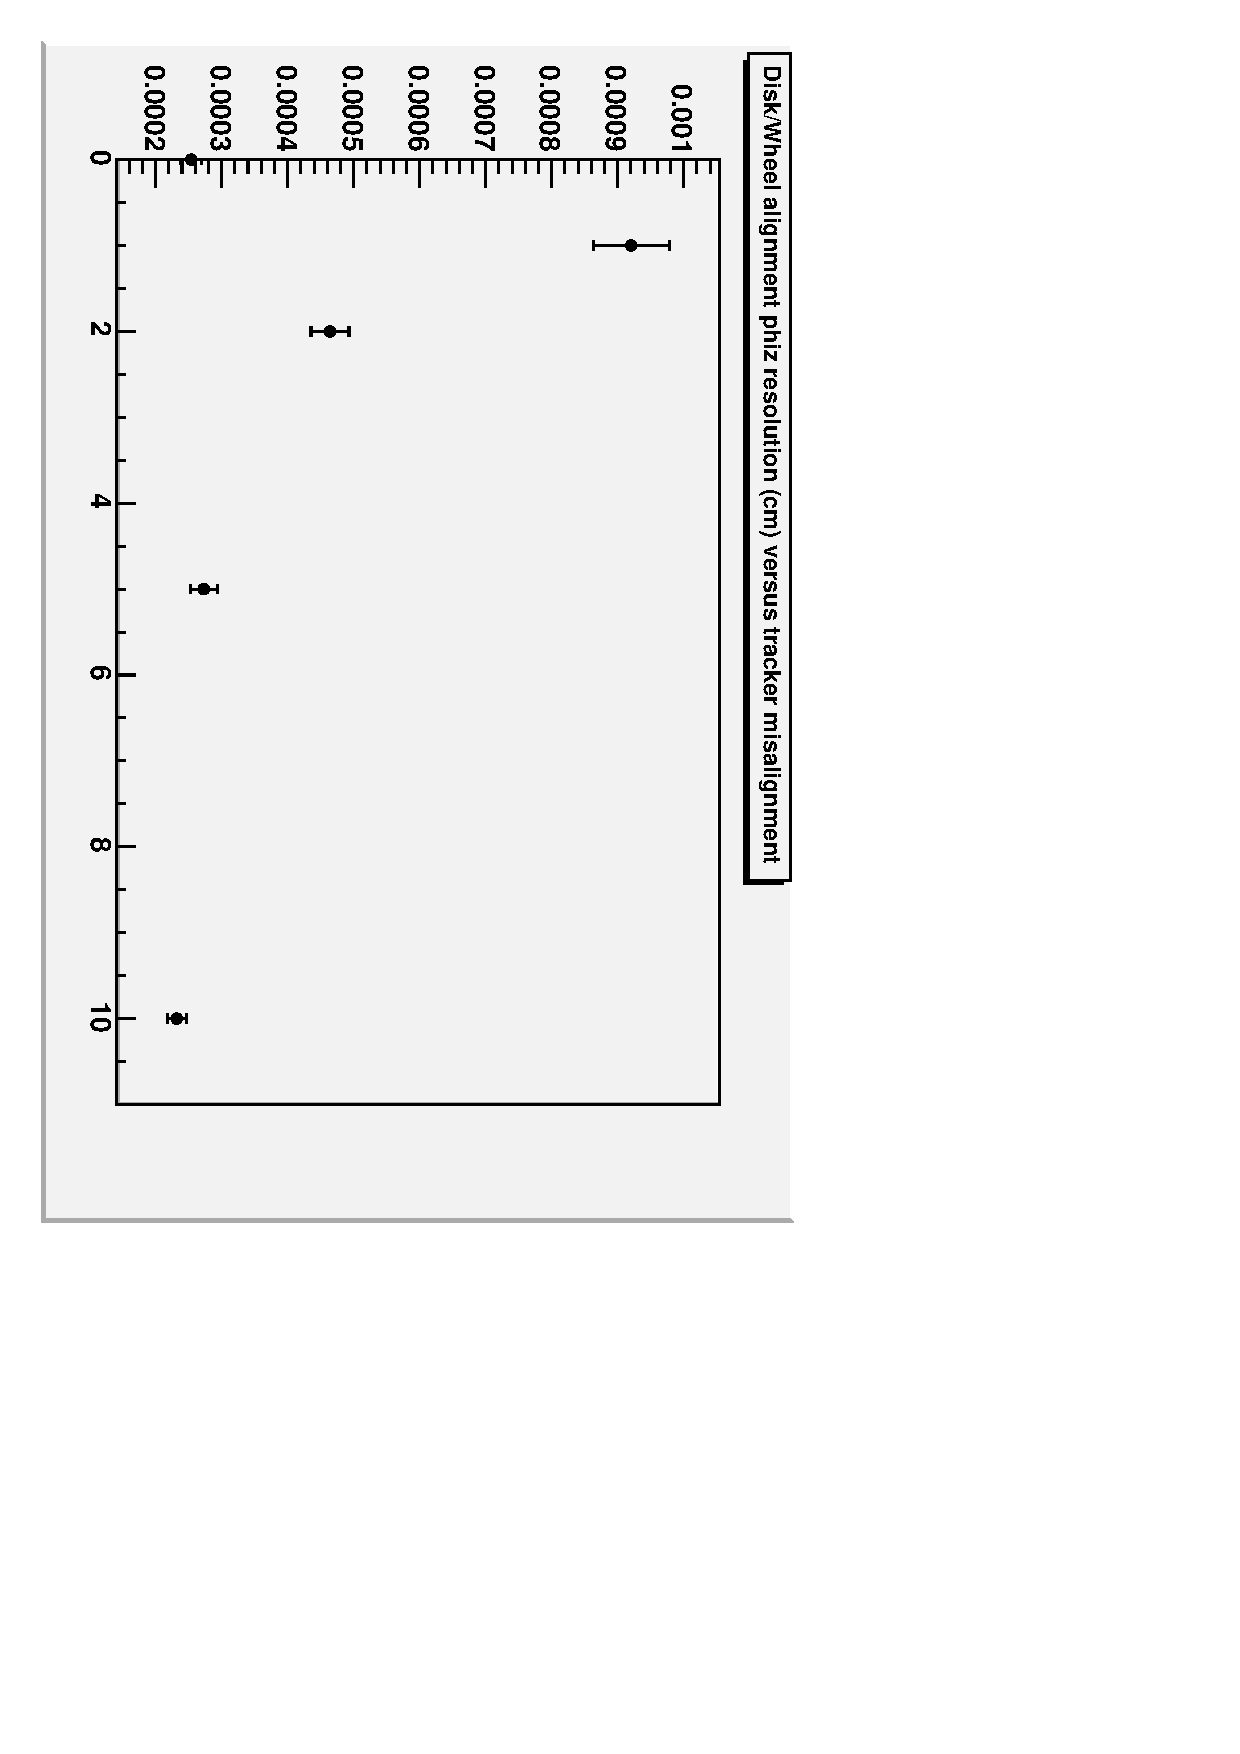
\includegraphics[height=0.6\linewidth, angle=90]{vstracker.pdf}
\end{center}

\vfill I need to find out how the misalignment scenarios affect
tracker APEs.  That might be the problem.  (It doesn't look like the
code is dividing by the scale factor, rather than multiplying.)

\end{frame}

\begin{frame}
\frametitle{Nominal case again (just a reminder): statistics study}
\begin{center}
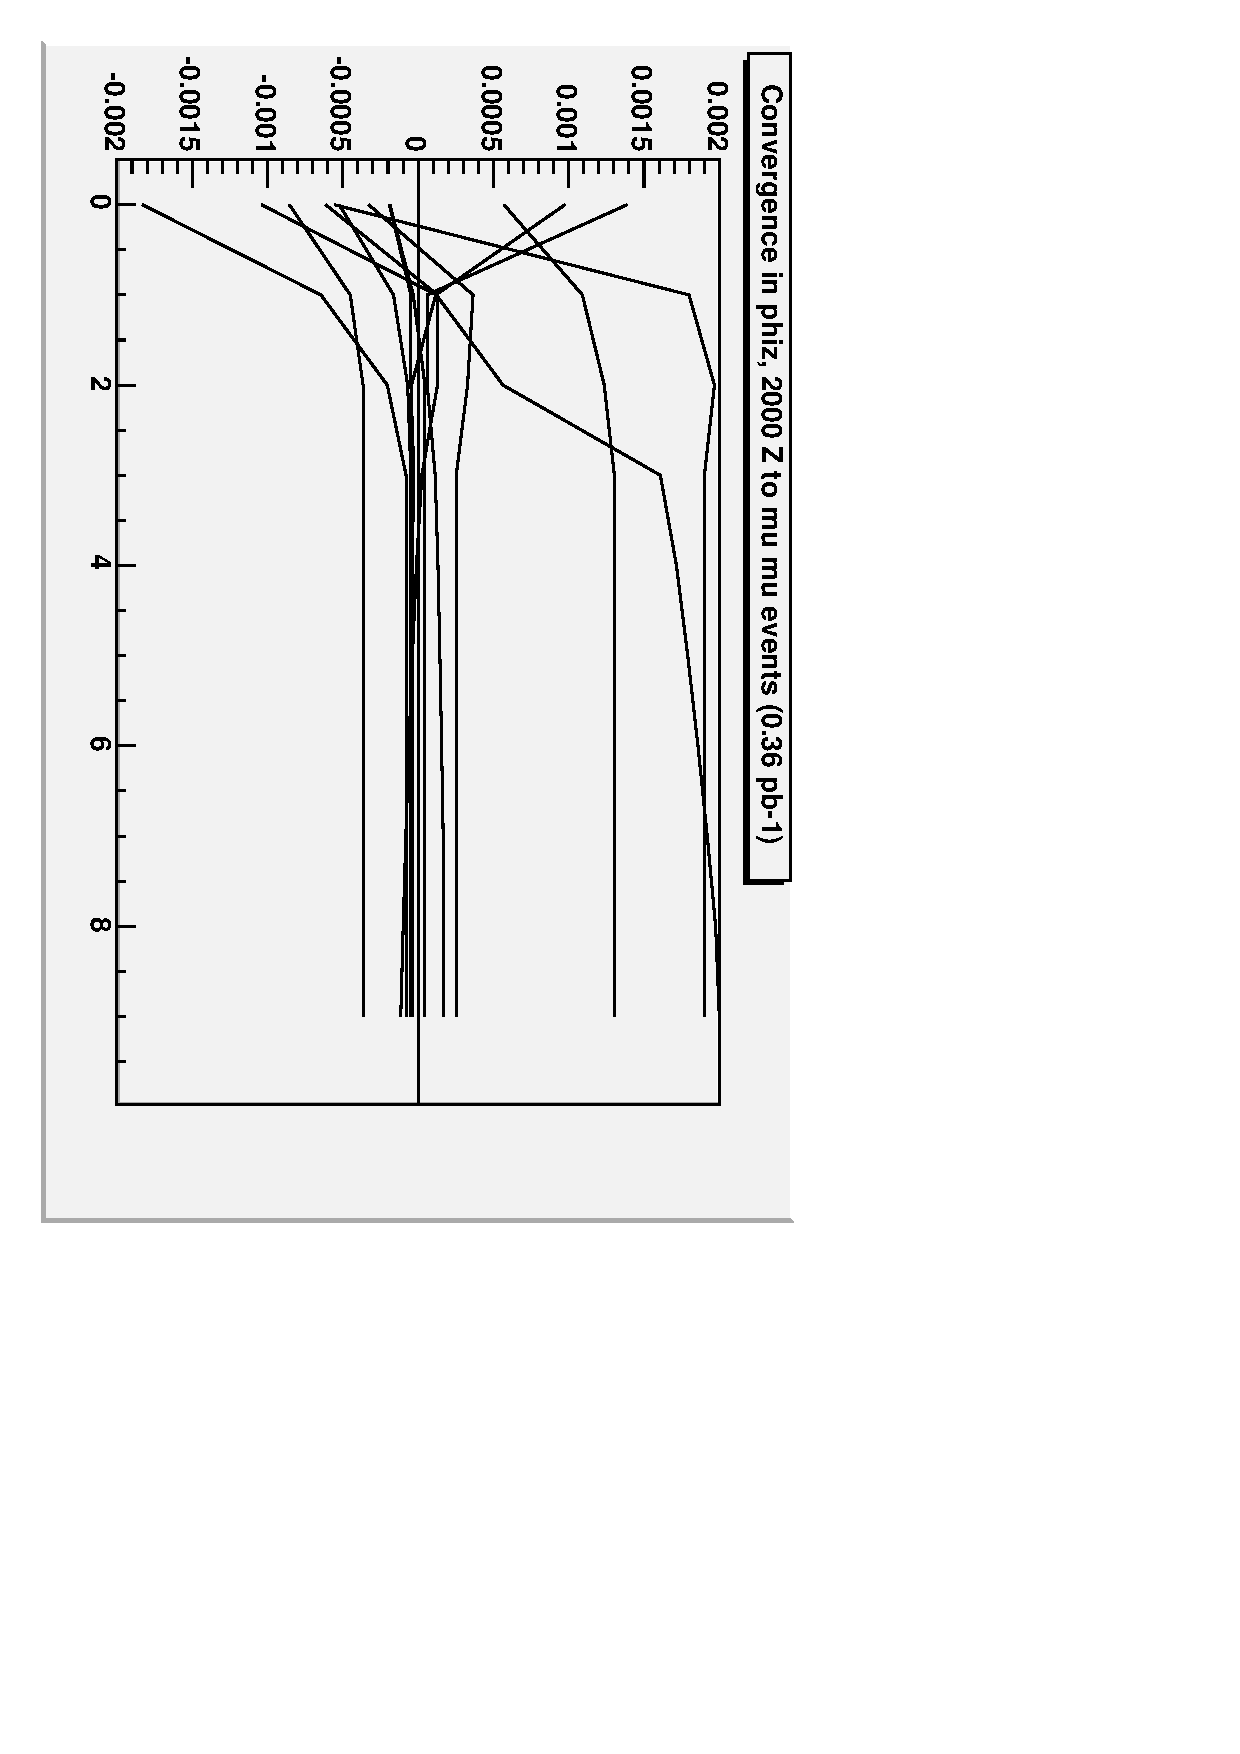
\includegraphics[height=0.8\linewidth, angle=90]{phiz_conv_2000.pdf}
\end{center}
\end{frame}

\begin{frame}
\frametitle{Half statistics}
\begin{center}
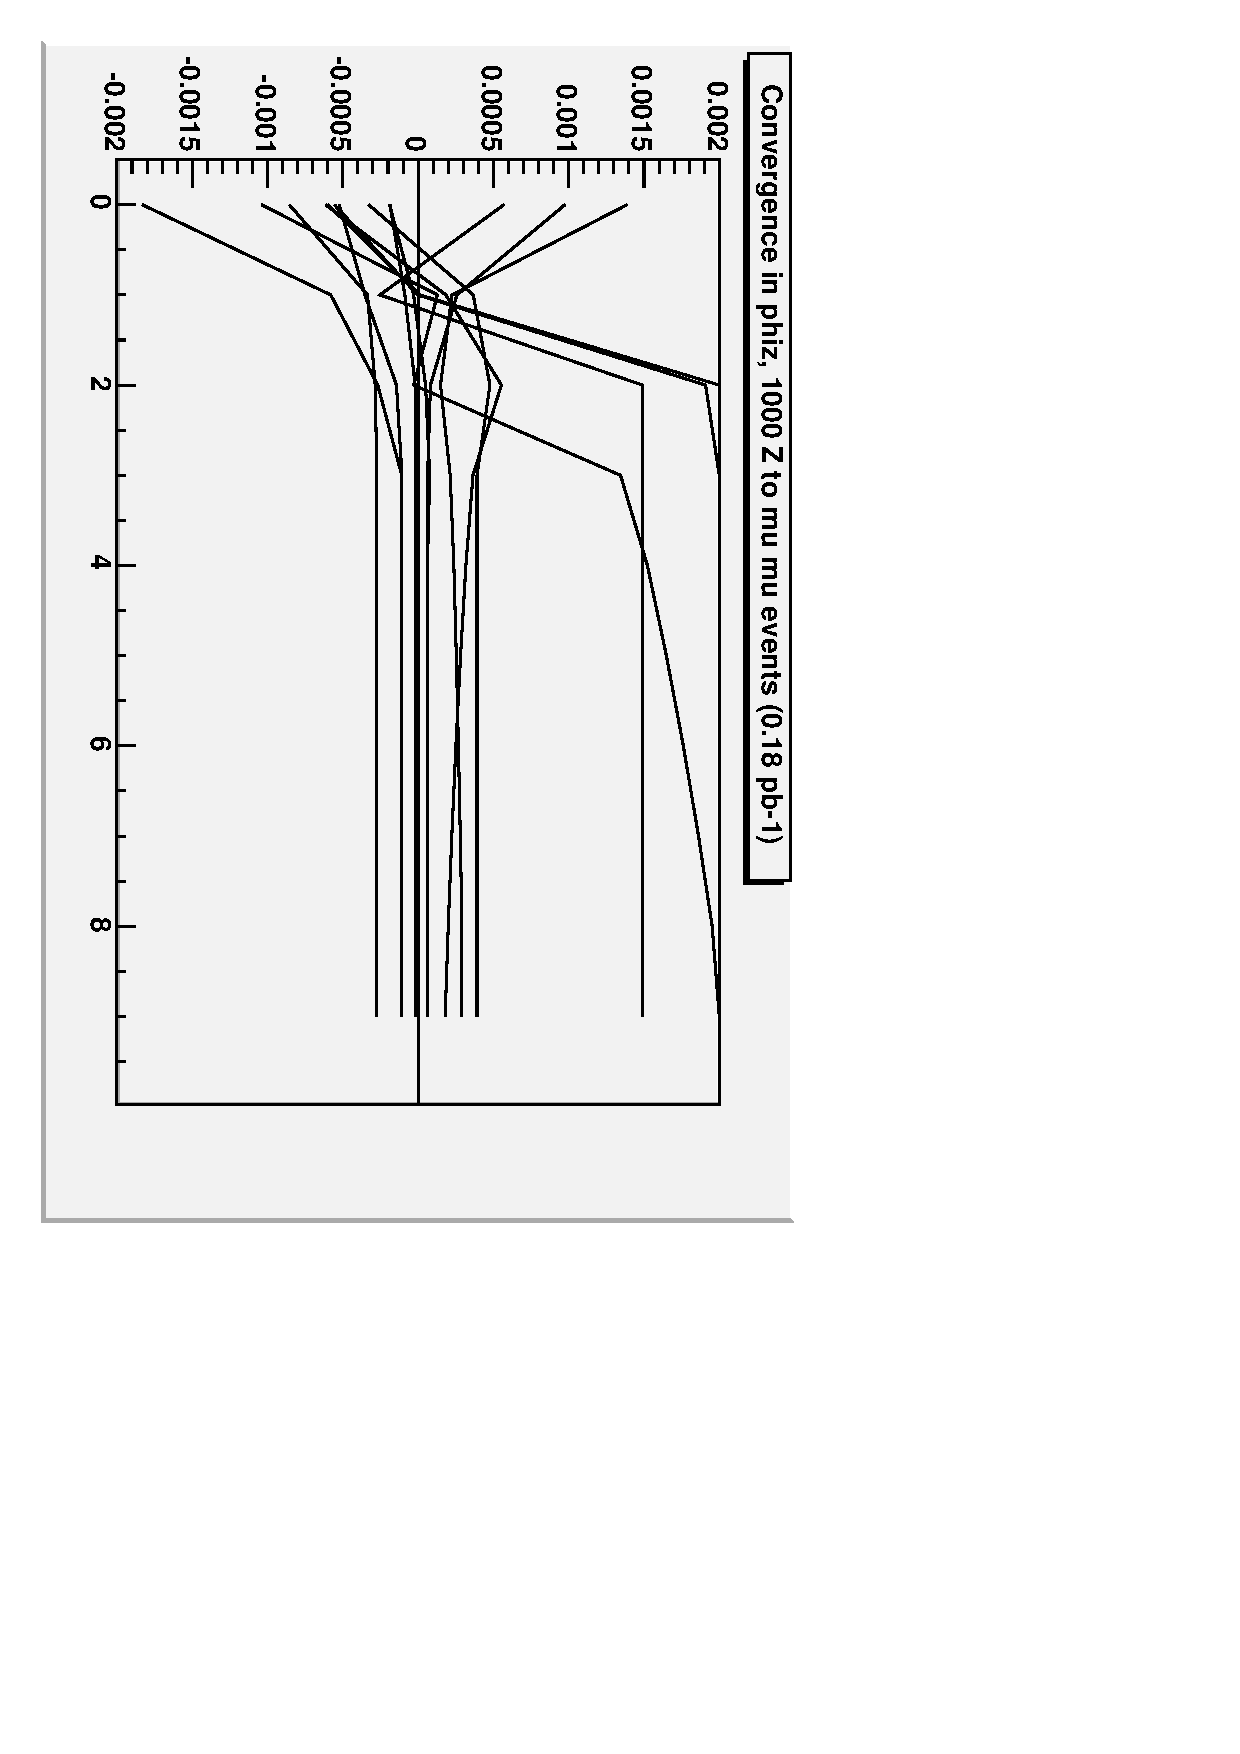
\includegraphics[height=0.8\linewidth, angle=90]{phiz_conv_1000.pdf}
\end{center}
\end{frame}

\begin{frame}
\frametitle{Quarter statistics}
\begin{center}
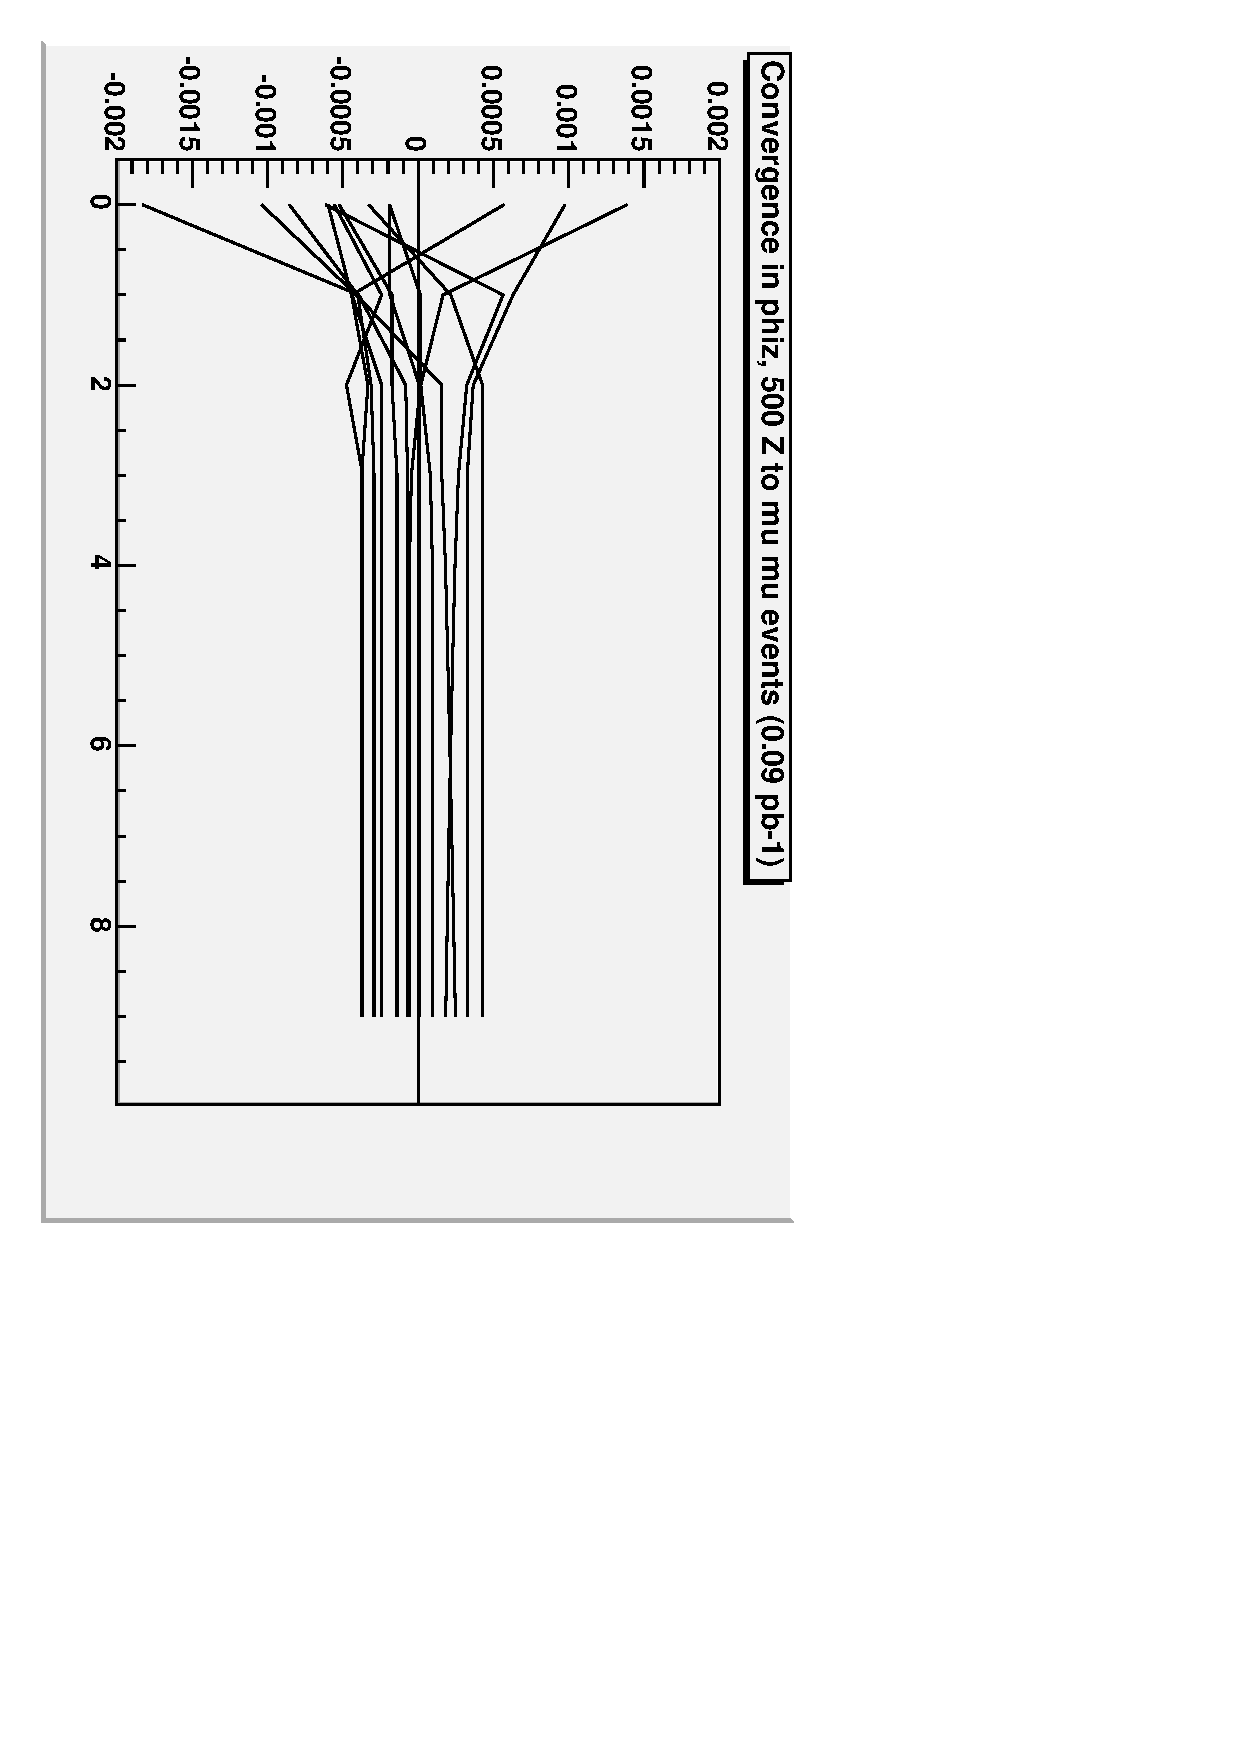
\includegraphics[height=0.8\linewidth, angle=90]{phiz_conv_500.pdf}
\end{center}
\end{frame}

\begin{frame}
\frametitle{Eighth statistics}
\begin{center}
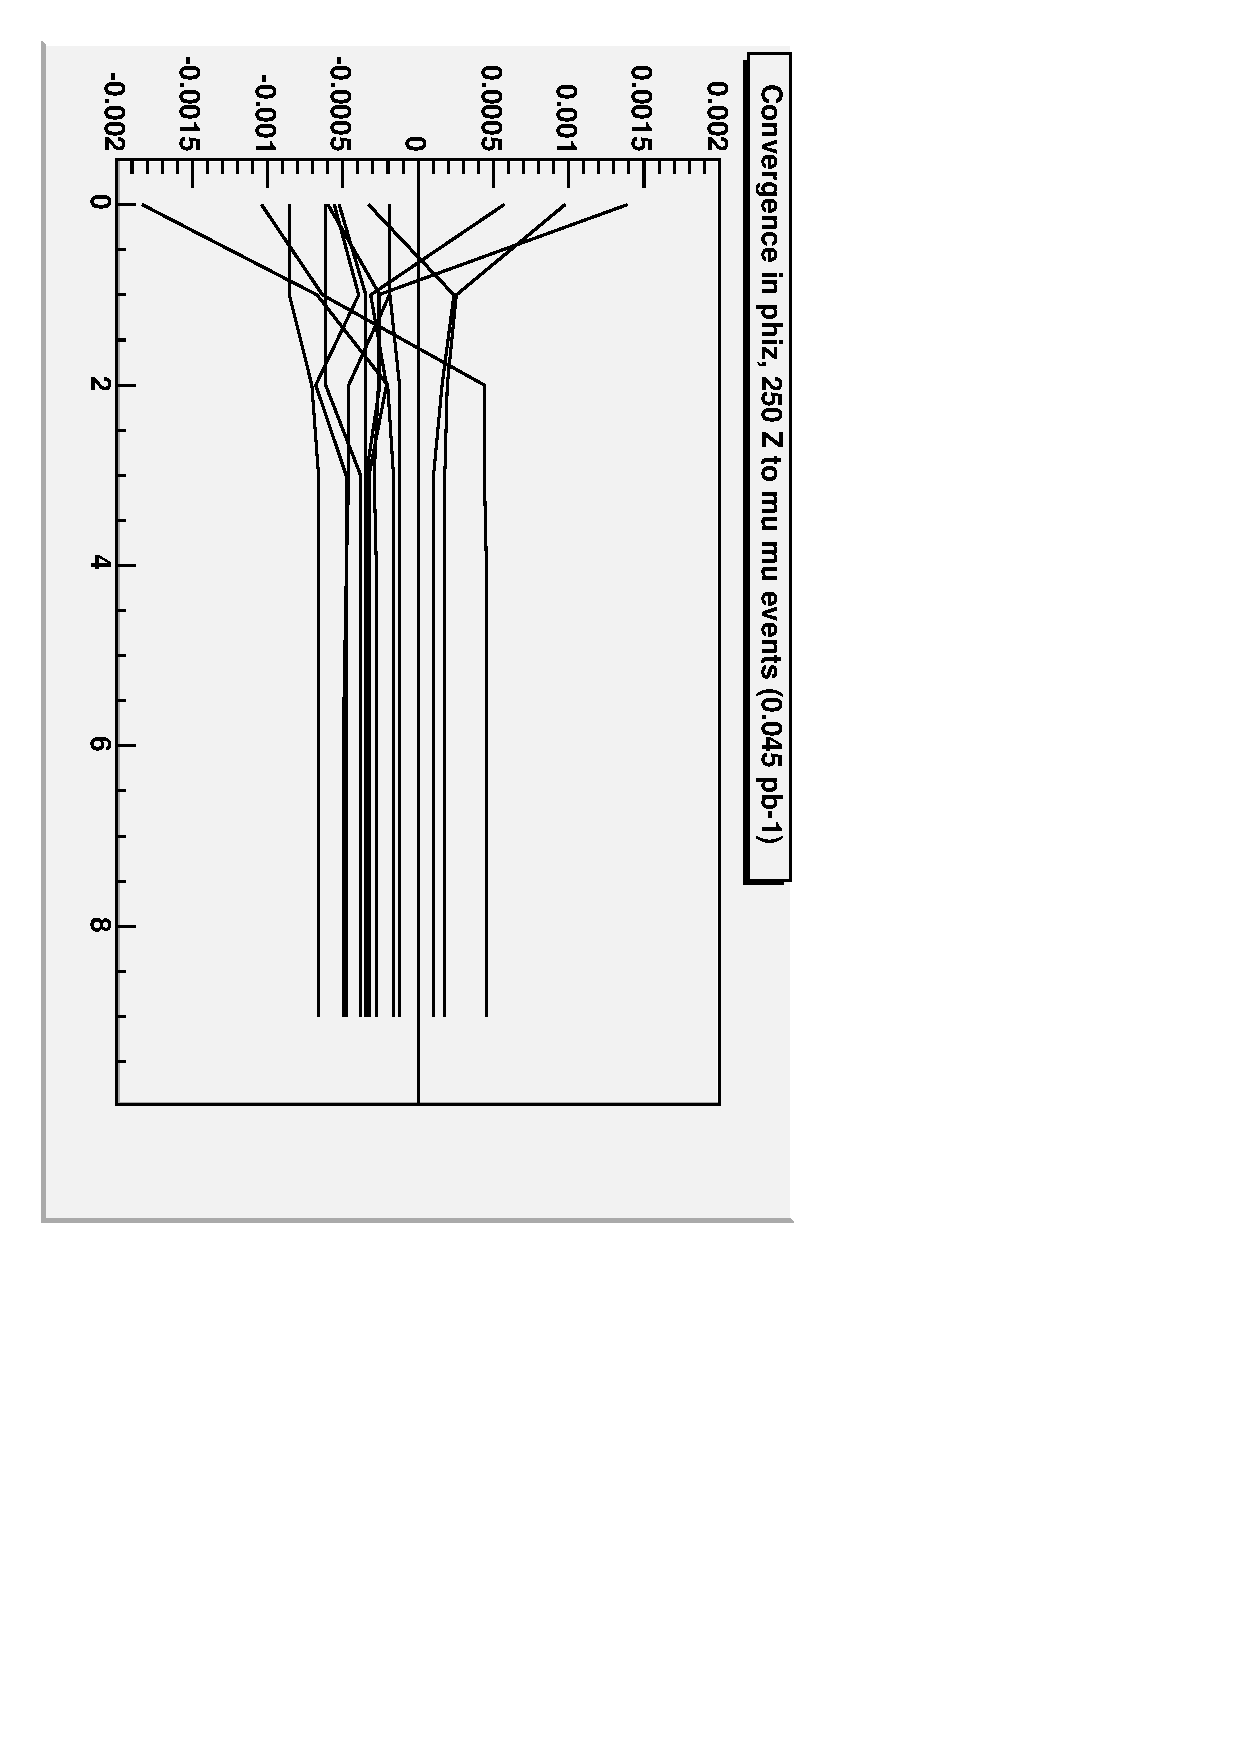
\includegraphics[height=0.8\linewidth, angle=90]{phiz_conv_250.pdf}
\end{center}
\end{frame}

\begin{frame}
\frametitle{I wouldn't claim to understand this yet.}

RMS of 13 disk/wheels times 10 trials, randomizing muon alignment with
each trial (but not tracker alignment).

\vfill
Events used in each simulation are independent.

\begin{center}
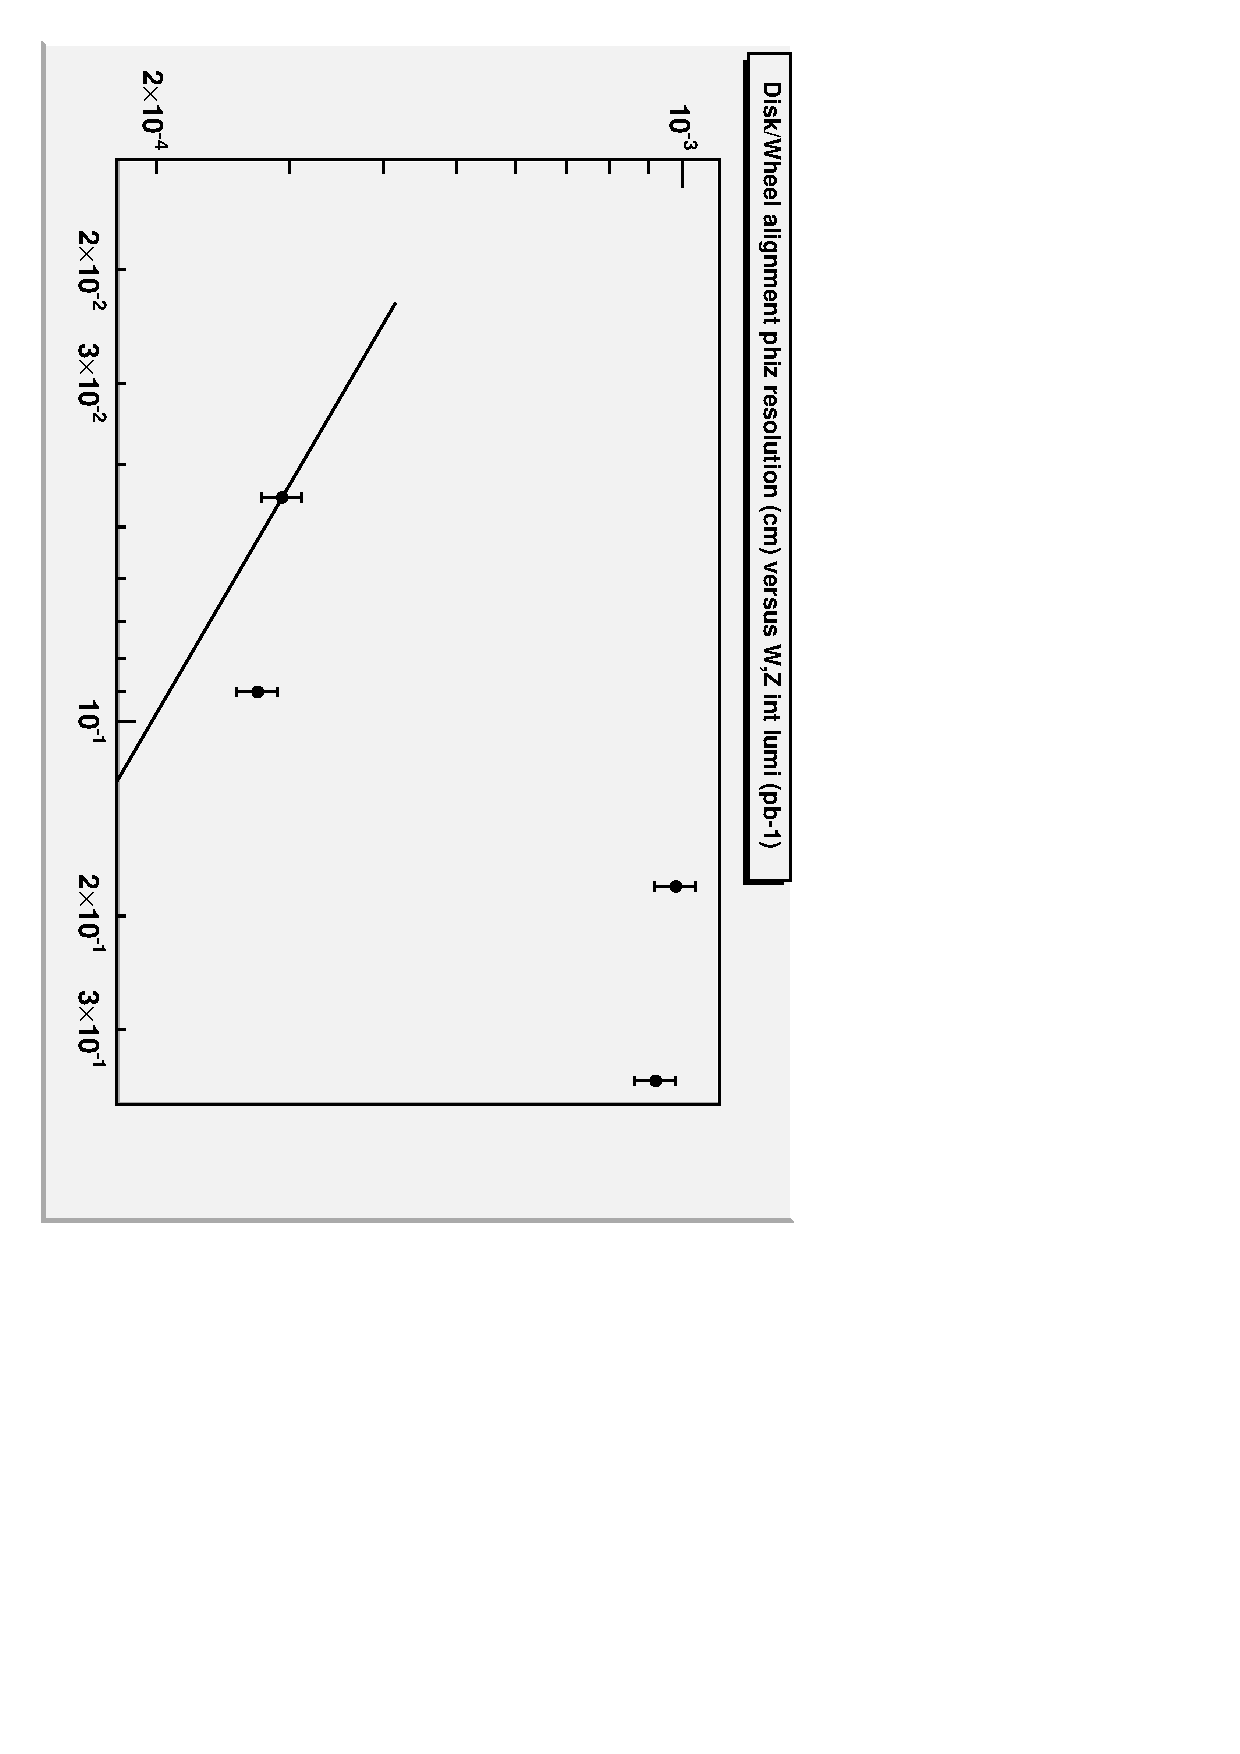
\includegraphics[height=0.6\linewidth, angle=90]{vsevents.pdf}
\end{center}

\vfill Those outliers affect the large-statistics trials most.

\label{numpages}
\end{frame}

\end{document}
